\documentclass{article}
\PassOptionsToPackage{numbers, sort&compress}{natbib}
\usepackage[dblblindworkshop,final]{neurips_2025}
\workshoptitle{2nd Workshop on Principles of Generative Modeling (PriGM)}
\makeatletter
\renewcommand{\@neuripsyear}{2026}
\renewcommand{\@neuripsordinal}{40th}
\makeatother
\usepackage[T1]{fontenc}
\usepackage[utf8]{inputenc}
\renewcommand{\ttdefault}{lmtt}
\usepackage{amsmath,amssymb,amsthm,booktabs,graphicx,longtable,microtype,float}
\usepackage{url}
\usepackage{hyperref}
\hypersetup{colorlinks=false,pdfborder={0 0 1},
  citebordercolor={0 1 0},urlbordercolor={0 1 1},linkbordercolor={1 0 0}}
\usepackage{orcidlink}
\hypersetup{pdfauthor={Kevin Lee},pdftitle={An Input Skip Can Reparameterize a VAE Without Improving the Generator},pdfsubject={},pdfkeywords={}}
\title{An Input Skip Can Reparameterize a VAE Without Improving the Generator}
\author{%
 Kevin Lee{\hypersetup{pdfborder={0 0 0}}\orcidlink{0009-0004-0388-9260}} \\
 [4pt] University of California at Los Angeles \\
 NASA Jet Propulsion Laboratory \\
 \texttt{kevinlee69720@g.ucla.edu}
}
\newcommand{\E}{\mathbb{E}}
\newcommand{\KL}{D_{\mathrm{KL}}}
\newtheorem{proposition}{Proposition}
\renewcommand{\bibfont}{\small}
\newcommand{\PrigmJobCount}{60}
\newcommand{\PrigmDatasetCount}{5}
\newcommand{\PrigmSeedCount}{3}
\newcommand{\PrigmCoreSHA}{37cc7445600eee541ee50aa580f6fdd6c0f37cf420074dbecc635c8d202946f5}
\newcommand{\PrigmWindowLength}{192}
\newcommand{\PrigmEvaluationSamples}{256}
\newcommand{\PrigmPriorSampleCount}{512}
\newcommand{\PrigmMaxMappedLogDensityError}{1}
\newcommand{\PrigmMaxMappedSampleMeanError}{\ensuremath{3.576\times10^{-7}}}
\newcommand{\PrigmMinMedianESS}{1}
\newcommand{\PrigmMaxAbsStabilityScoreChange}{0.2616}
\newcommand{\PrigmMaxAbsReplicateScoreChange}{0.07691}

\newcommand{\PrigmCombinedSHA}{1a20c43a29e640ff590e4c0f553bc7f08f2fad46fe6e2dab0e18806e20104fee}

\hypersetup{pdfsubject={PriGM core SHA256: \PrigmCoreSHA; combined SHA256: \PrigmCombinedSHA}}
\begin{document}
\maketitle

\begin{abstract}
An input skip can make a model reconstruct its input more accurately without improving its distribution of new samples. For a Gaussian variational autoencoder (VAE) with constant input skip $0\leq\alpha<1$, rescaling the residual decoder by $b=1-\alpha$ and its variance by $b^2$ preserves the joint distribution of observations and latent variables. Reconstruction mean squared error (MSE) becomes $b^2$ times its original value, while generative scores retain their values. Separate training can produce different generators because the optimizer acts on different parameter coordinates. In a Gaussian experiment with known density, changing skip and observation variance together reduces MSE but worsens both energy score and an importance weighted estimate of negative log density. On seven annual \mbox{Deep-ocean} Assessment and Reporting of Tsunamis (DART) records, energy score comparisons at the same observation variance vary in direction on four original records and favor the skip on three records from 2018. Probabilistic principal component analysis (PPCA) gives lower mean energy scores than every neural DART fit. Estimating observation variance from training reconstruction error, with the encoder and decoder kept the same, can also worsen this score. Reconstruction error alone is insufficient to assess generation.
\end{abstract}

\section{Introduction}
A variational autoencoder (VAE) reconstructs an observation through an encoder and a decoder, and generates new observations by sampling a latent variable $z$ from its prior and then sampling from the decoder $p(x\mid z)$ \citep{KingmaWelling2014AutoEncodingVB}. An input skip adds a scalar multiple of the observation directly to its reconstruction: $\hat x=f_\theta(z)+\alpha x$. As the coefficient $\alpha$ grows, the input itself can account for more of the reconstruction. A smaller error can therefore arise without a better distribution of new samples.\footnote{Available at: \url{https://github.com/magnaprog/vae-skip-reparam}.}

For constant $0\leq\alpha<1$ and Gaussian noise, rescaling the decoder and noise preserves the model's joint distribution and multiplies reconstruction mean squared error (MSE) by $(1-\alpha)^2$. This identity relates two representations of one generator. Separate training can give different generators because Adam and gradient clipping act in different parameter coordinates \citep{KingmaBa2015Adam,Dinh2017SharpMinima}. Comparisons at the same observation variance distinguish these training outcomes from the algebraic reduction in error. The input skip considered here differs from the links of Dieng et al., which carry $z$ into decoder layers to encourage latent dependence \citep{Dieng2019SkipVAE}.

National Oceanic and Atmospheric Administration (NOAA) Deep-ocean Assessment and Reporting of Tsunamis (DART) records provide an application in which both oscillations and changes in mean level matter. Their HEIGHT variable expresses bottom pressure as equivalent water column height \citep{NDBCDARTDescription,Meinig2005DARTII}. Earlier work used an adaptive input skip and iterative reconstruction at station 23461 in 2022 \citep{Lee2024DARTPredecessor}. Here a constant skip isolates the effect of feeding the input into reconstruction. The models generate windows of 192 consecutive routine observations, and evaluation compares their distributions with later data. Observation variance is varied separately because it sets the relative weight of reconstruction and Kullback--Leibler (KL) divergence during training \citep{Rybkin2021CalibratedDecoders}.

\section{Input skip and generative evaluation}
Let $x\in\mathbb{R}^d$, $0\leq\alpha<1$, and $b=1-\alpha$. The encoder $q_\phi(z\mid x)$ approximates the posterior and supplies latent samples for importance sampling. Reconstruction MSE is $d^{-1}\|x-f_\theta(\E_q Z)-\alpha x\|^2$. If $f_\theta=b g_\theta$, then $x-f_\theta(z)-\alpha x=b(x-g_\theta(z))$, so squared error scales by $b^2$, equal to $0.04$ at $\alpha=0.8$. Dividing reconstruction MSE by $b^2$ gives MSE in observation coordinates.

The implicit generative model is $X=\alpha X+f_\theta(Z)+\epsilon$, where $Z\sim\mathcal{N}(0,I)$ and $\epsilon\sim\mathcal{N}(0,\sigma_r^2I)$ are independent. Solving for $X$ gives its conditional density and a rule for generating samples:
\begin{equation}
 p_\alpha(x\mid z)=b^d\mathcal{N}(bx;f_\theta(z),\sigma_r^2I),
 \qquad X=\frac{f_\theta(Z)+\epsilon}{b}.
\label{eq:density}
\end{equation}
Thus the conditional observation mean is $g_\theta(z)=f_\theta(z)/b$ and observation variance is $\sigma_x^2=\sigma_r^2/b^2$. The evidence lower bound (ELBO) is a variational lower bound on $\log p_\alpha(x)$.

\begin{proposition}
\label{prop:equivalence}
Let a fitted model have conditional density $\mathcal{N}(x;g_\theta(z),\sigma_0^2I)$, with $\sigma_0^2>0$, prior $p(z)=\mathcal{N}(0,I)$, and encoder $q_\phi(z\mid x)$. Map its decoder to $f=b\,g_\theta$ and residual variance to $\sigma_r^2=b^2\sigma_0^2$, where $b>0$. This preserves the joint distribution of $(X,Z)$, marginal $p_\alpha(x)$, exact posterior $p_\alpha(z\mid x)$, ELBO for the common encoder, and importance weights $p(x\mid z)p(z)/q_\phi(z\mid x)$ for common samples. Reconstruction MSE scales by $b^2$.
\end{proposition}

The proof follows by changing variables from $x$ to $bx$ and including the density's Jacobian factor; Appendix A gives the details. Table~\ref{tab:conditions} separates skip and observation variance into four training conditions. Separate fits use the same Adam learning rate, numerical stabilizer, and total gradient norm limit in residual coordinates. These settings permit different training paths even when the initial observation means agree.

\begin{table}[t]
\centering
\caption{Skip and variance conditions. A/C use observation variance $\sigma_0^2$ and B/D use $25\sigma_0^2$, where $25=1/(1-0.8)^2$. A/D omit the skip and B/C use $\alpha=0.8$. The original A/B comparison changes both skip and observation variance.}
\label{tab:conditions}
\begin{tabular}{lcc}
\toprule
Skip coefficient & Base variance: $\sigma_0^2$ & High variance: $25\sigma_0^2$\\
\midrule
$\alpha=0$ & No skip/base (A) & No skip/high (D)\\
$\alpha=0.8$ & Skip/base (C) & Skip/high (B)\\
\bottomrule
\end{tabular}
\end{table}

Each condition uses one sample from the encoder distribution to estimate the expectation in the negative ELBO,

\begin{equation}
\mathcal{L}_\alpha
=-\E\bigl[\log p_\alpha(x\mid z)\bigr]+\KL\bigl(q_\phi(z\mid x)\Vert p(z)\bigr),
\qquad z\sim q_\phi(z\mid x),
\label{eq:objective}
\end{equation}

with the normalized density in Eq.~\ref{eq:density} and KL coefficient $\beta=1$. The appendix relates this objective to squared reconstruction error.

\section{Experiments}
\subsection{Data}
The Gaussian experiment has eight independent normal latent factors, orthogonal sinusoidal loadings in 192 coordinates, and isotropic noise of standard deviation 0.25. NOAA describes instrument measurements every 15 s and routine T=1 values 15 minutes apart \citep{NDBCDARTDescription,Meinig2005DARTII,NDBC2023WebDataGuide}. The analysis uses T=1 observations from NOAA annual files \citep{NDBCDARTHistoricalData}, without despiking, detrending, or detiding. Each window has 192 samples at 900 s spacing, spanning 47 h 45 min.

Four original records use equal window weights; three training partitions span deployments. Three records from 2018 use overlapping test windows within NOAA deployment periods. The choice of 44402/2018 followed examination of its 2016 file. Stations 21415 and 21418 were chosen in identifier order among eligible records before neural results. Their windows start every four hours UTC with calendar 60/20/20 splits and exclusions of two days on each side of each split date. Each of six UTC start hours has total weight $1/6$. The appendix gives station records, counts, and selection criteria.

\subsection{Models and comparisons}
Each record uses four conditions and three training seeds. Within each 2018 record and seed, conditions share initial observation means, minibatches, and encoder sampling noise. Encoders use 16 latent coordinates; PPCA has at most 16 loading directions \citep{TippingBishop1999ProbabilisticPCA}. PPCA determines base variance, using a validation grid for 2018 before neural fitting. Original models use weights chosen by validation. All 36 models for 2018 complete 10,000 Adam steps, with evaluation of final weights and weights chosen by validation.

\subsection{Evaluation}
The energy score evaluates agreement between a model distribution and observations using Euclidean distances \citep{GneitingRaftery2007ProperScoringRules}. Its name comes from energy statistics and an analogy with potential energy \citep{RizzoSzekely2016EnergyDistance}. For each observation, it subtracts half the mean distance between independent model samples from their mean distance to that observation. Lower values are better. DART evaluation uses three independent streams of 1,024 generated windows. Conditions share latent prior samples and standard normal noise. Scores use full windows, windows after subtraction of their own means, or time differences across several lags, all in coordinates standardized by the training mean and standard deviation. Mean subtraction removes each window's level; time differences measure changes over the chosen lags. Differences compare conditions with the same training seed. Medians and full ranges across three seeds describe variation between fits, with Monte Carlo variation given separately. Negative importance weighted (IW) log density estimates use $K=256$ and three streams \citep{BurdaGrosseSalakhutdinov2016IWAE}. Low effective sample size (ESS) limits their interpretation.

\subsection{Observation variance estimation}
With encoder and decoder weights unchanged, observation variance is estimated as
\begin{equation}
\hat v=\frac{1}{d}\sum_{i\in\mathrm{train}}w_i\,\widehat{\E}_{q_\phi(z\mid x_i)}\|x_i-g_\theta(z)\|^2
\label{eq:variance_refit}
\end{equation}
from three independent streams of 32 posterior samples per training window, with training weights that sum to one. This minimizes the sampled expected Gaussian reconstruction term, including its log normalizer. Rybkin et al.\ also update encoder and decoder weights \citep{Rybkin2021CalibratedDecoders}. Here only observation variance changes for evaluation and sampling.

\section{Results}
\subsection{Synthetic Gaussian experiment}
The original comparison changes both skip and observation variance, from no skip at base variance to skip at high variance (A/B). Across three runs, median reconstruction MSE falls from 0.0616 to 0.00368, while median estimated negative IW log density rises from 0.133 to 1.201 nats per coordinate and median energy score rises from 5.723 to 7.123. Thus both generative scores worsen despite the smaller reconstruction error. At base observation variance, the skip model (C) gives median MSE 0.00250 and median negative log estimate 0.137, compared with 0.125 for the known generating Gaussian and 0.127 for PPCA. These are separate fits; rescaling the decoder and noise of a fitted model from A to C would preserve its generator and exact proper scores.

The high observation variance in B/D sets a noise floor before training. Its value, $25\sigma_0^2=1.53929$, exceeds the data variance along 185 of 192 covariance directions. Since independent observation noise gives $\operatorname{Cov}(X)=\operatorname{Cov}(g(Z))+\sigma_x^2I\succeq\sigma_x^2I$, those models necessarily have excess variance in these directions. Increasing decoder flexibility leaves this noise contribution in place. Score differences also depend on fitting and, for log estimates, approximate inference.

\begin{figure}[t]
\centering
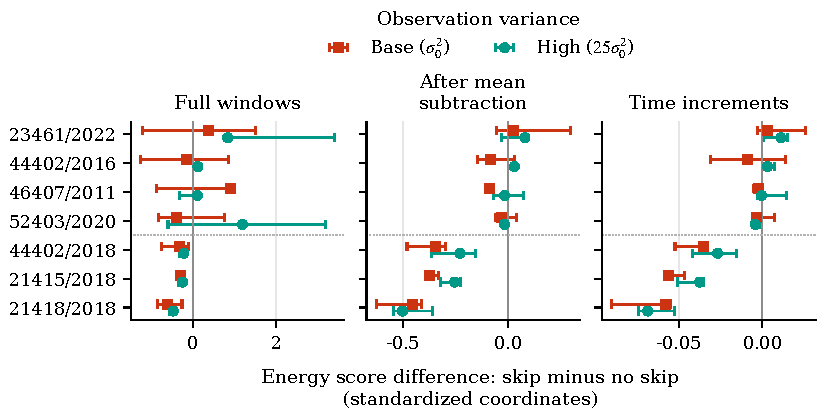
\includegraphics[width=\linewidth,height=0.81\textheight,keepaspectratio]{figures/presentation/reconstruction_generation.pdf}
\caption{DART energy score differences at the same observation variance. Squares show skip minus no skip at base variance $\sigma_0^2$ (C-A), and circles at high variance $25\sigma_0^2$ (B-D). Negative values favor the skip. Columns use full windows, subtraction of each window's mean, and time increments in standardized coordinates. Points and bars give medians and full ranges of differences across three training seeds, after averaging three sampling streams within each fit. Table~\ref{tab:dart_contrasts} gives sampling variation. Original records use equal window weights and network weights chosen by validation; 2018 cases use UTC start hour weights and final network weights.}
\label{fig:comparison}
\end{figure}

\subsection{DART case studies}
Energy score differences take both signs across the four original records. Subtracting each window's mean reverses the median C-A sign for 46407/2011, showing how mean level affects the comparison (Figure~\ref{fig:comparison}). For all three 2018 cases, the skip lowers all three mean energy scores at both observation variances. Within 21415/2018 and 21418/2018, energy score differences for full windows take both signs across intervals of 14 days and training seeds (Table~\ref{tab:dart_blocks}). PPCA has lower mean energy score than every neural fit on all seven cases and three scores, including at the same observation variance (Table~\ref{tab:dart_energy}). The leading 16 covariance eigenvectors account for almost all training variance, making PPCA a useful linear baseline (Appendix~\ref{sec:reference_distributions}). Its advantage combines differences in model class and fitting procedure.

\subsection{Estimating observation variance}
With encoder and decoder weights unchanged, the variance estimate from training error increases variance in all 42 fits trained at $\sigma_0^2$ and decreases it in all 42 trained at $25\sigma_0^2$. All three mean energy scores improve in the first group and worsen in the second (Figure~\ref{fig:dart_variance_refit}). After averaging streams within each fit, the change in half the mean distance between model samples exceeds the change in mean distance to observations in absolute magnitude. This subtracted term therefore determines the direction of every score change (Appendix~\ref{sec:variance_reset}). Reducing the Gaussian reconstruction loss on training windows can worsen energy score on test windows.

\section{Conclusion}
For a Gaussian VAE with a constant input skip, exact rescaling can make reconstruction MSE arbitrarily small while preserving the generator. Separate DART fits give energy score differences of both signs, and PPCA has lower mean scores than every neural fit. Reconstruction error therefore needs to be interpreted together with observation variance and generative scores.

\clearpage
\bibliographystyle{unsrtnat}
\bibliography{references}

\clearpage
\appendix
\setlength{\LTcapwidth}{\linewidth}
\section{Density, MSE, and energy score}
Consider an objective with a sum of squared residuals, $\E\|x-f_\theta(z)-\alpha x\|^2+\beta_\alpha R$, where $R=\E_x\KL(q_\phi(z\mid x)\Vert p(z))$. The sum is over observation coordinates, before division by $d$. When $f_\theta=b g_\theta$,
\begin{equation}
\frac{\E\|x-f_\theta(z)-\alpha x\|^2+\beta_\alpha R}{b^2}
=\E\|x-g_\theta(z)\|^2+\frac{\beta_\alpha}{b^2}R.
\label{eq:scale}
\end{equation}
At $\alpha=0.8$, the reconstruction term is multiplied by $0.04$, making $\beta_\alpha/b^2$ equal to $25\beta_\alpha$. Keeping the KL coefficient constant therefore gives KL greater weight relative to squared error. Training minimizes the negative ELBO computed from the normalized density, with KL coefficient one. Dropping terms constant in the parameters during training and multiplying by $2\sigma_r^2$ gives the sum of squared residuals with KL coefficient $2\sigma_r^2$. If squared residuals are averaged over coordinates, the equivalent coefficient is $2\sigma_r^2/d$. Conversely, expressing negative ELBO as the sum of a multiple of MSE and KL gives MSE coefficient $d/(2\sigma_r^2)$.

\begin{proof}[Proof of Proposition~\ref{prop:equivalence}]
The change of variables $r=bx$ has Jacobian determinant $b^d$. In the mapped model, $r$ has conditional Gaussian mean $b\,g(z)$ and covariance $b^2\sigma_0^2I$. Multiplying its density by the Jacobian gives $\mathcal{N}(x;g(z),\sigma_0^2I)$. The unchanged prior then gives the same joint distribution, marginal, and exact posterior. With the same encoder the ELBO is preserved, and with the same latent draws each importance weight is preserved. Finally, $\|b x-b g(z)\|^2=b^2\|x-g(z)\|^2$ holds for each $z$, including the common encoder mean, and also after averaging over the common encoder distribution.
\end{proof}

Reconstruction MSE evaluates the decoder at $z=\E_q Z$. With a nonlinear decoder, this error can be larger or smaller than MSE averaged under the encoder distribution. That expectation enters the Gaussian reconstruction term in the ELBO. Both scale by $b^2$ under the mapping. Multiplication by this positive constant preserves error rankings and therefore any anomaly rankings based on that error. A threshold at the mean error plus a constant multiple of its standard deviation scales by the same factor. Classification decisions are preserved. These results concern two forms of one model. For separate fits, reconstruction MSE measures reproduction of the input; evaluating generation also requires samples or densities from the generator.

Averaging Eq.~\ref{eq:density} over the latent prior gives the marginal density. This integral differs from decoding one encoder mean. The mapping preserves every strictly proper score of the marginal, including log score and, for distributions with finite first moments, energy score \citep{GneitingRaftery2007ProperScoringRules}. A finite importance estimate also retains its value when both forms use the same encoder distribution and latent samples. For affine decoders, which are linear maps with an offset, the two Gaussian models have the same joint distribution and exact posterior.

The study concerns a constant scalar $\alpha<1$. The singular case $\alpha=1$, input dependent skips, and matrix coefficients each require separate analysis. The implicit generator samples noise once and solves for $X$. At $\alpha=0.8$ with residual variance one, its conditional variance is 25. An autoregressive process of order one, AR(1), repeatedly multiplies the previous state by 0.8 and adds constant forcing and fresh independent noise. With noise variance one, that process has stationary variance $1/(1-0.8^2)\simeq2.778$.
Other VAE constructions can also weaken dependence on latent variables. Attention that passes information without sampling a latent variable can bypass a stochastic latent representation \citep{Bahuleyan2018VariationalAttention}. Equal ELBO values can accompany different representations \citep{Alemi2018FixingBrokenELBO}. Analyses of linear conditional and hierarchical VAEs relate posterior collapse to correlation between input and output and to encoder variance that is learned during training \citep{Dang2024BeyondVanilla}. Dieng et al.\ add residual links from $z$ into the decoder to encourage dependence of $p(x\mid z)$ on the code \citep{Dieng2019SkipVAE}. Feeding $x$ into the reconstruction supplies a route that can ignore $z$, while generation still uses $z$ and noise. For the constant input skip here, the rescaling in Eq.~\ref{eq:density} gives the density explicitly.

Under suitable assumptions on regularization and corruption noise, regularized autoencoders can recover derivatives of the data log density \citep{AlainBengio2014WhatRegularizedAutoEncodersLearn}. Those results describe information in a learned reconstruction function. Here Eq.~\ref{eq:density} specifies the generative density directly, with normalization supplied by the affine transformation.

As a scalar check of the scoring definitions, take $X\sim\mathcal{N}(0,1)$, $f=0$, and $\sigma_r^2=1$. Increasing $\alpha$ from zero to 0.8 reduces expected reconstruction MSE from one to 0.04. Expected negative log likelihood for the normalized density rises from approximately 1.419 to 2.548 nats. These are population expectations.

For each test window, $K$ latent samples from the encoder distribution give the estimate
\begin{equation}
\widehat\ell_K(x)=\log\left[\frac1K\sum_{k=1}^K
\frac{p_\alpha(x\mid z_k)p(z_k)}{q_\phi(z_k\mid x)}\right],
\qquad z_k\sim q_\phi(z\mid x).
\end{equation}
The expectation of this estimate is at most $\log p_\alpha(x)$, although a single realization can exceed it. At finite $K$, its value depends on both the encoder sampling distribution and the marginal density. The proper log score concerns exact marginal density. Log weights are calculated and accumulated in double precision after single precision neural calculations. Effective sample size, $(\sum w_k)^2/\sum w_k^2$, measures concentration of the importance weights. When the encoder poorly approximates the posterior, a few samples can carry almost all the importance weight. Comparing fits changes both the density being estimated and the distribution used to sample latent values.

For normalization $u=(h-m)/s$, with mean $m$ and scale $s$ estimated from training rows, log density in meter coordinates is $\log p_H(h)=\log p_U(u)-d\log s$. Log density comparisons use standardized DART coordinates and original Gaussian coordinates. All logarithms are natural, hence their units are nats. A density for the complete time series would also need a model of dependence between windows.

With observation mean $g(z)=f(z)/b$ and variance $v=\sigma_r^2/b^2$, negative ELBO per coordinate is
\begin{equation}
\frac{\mathcal L_\alpha(x)}{d}=\frac12\log(2\pi v)+\frac{\E_q\|x-g(Z)\|^2}{2dv}+\frac{\KL(q\Vert p)}d.
\label{eq:elbo_components}
\end{equation}
Multiplying $v$ by 25 increases the first term by $\log(25)/2$. The expectation in the second term uses the encoder distribution; substituting the error from the encoder mean would change the objective. In expectation, the IW lower bound with $K$ samples is at least as tight as the ELBO. The improvement varies between models, so differences in that improvement can have either sign. For any given set of log weights, Jensen's inequality gives $\widehat\ell_K-K^{-1}\sum_k\log w_k\geq0$. This difference compares the log of the mean importance weight with the mean log weight, using the same samples. Error relative to exact marginal log density remains unknown, and replacing sampled log ratios with analytic KL gives a different comparison.

For independent samples $y_1,\ldots,y_M$ from the model's marginal distribution, the Gneiting and Raftery energy score has the estimator
\begin{equation}
\widehat{\mathrm{ES}}(x)=\frac1M\sum_i\|y_i-x\|_2
-\frac{1}{M(M-1)}\sum_{i<j}\|y_i-y_j\|_2.
\end{equation}
The second term uses distinct sample indices. If samples are identically distributed and independent of each other and the evaluation observation, the estimate is unbiased for population energy loss. That loss is strictly proper for distributions with finite first moments \citep{GneitingRaftery2007ProperScoringRules}: its expectation is uniquely minimized by the true distribution. Finite ensembles introduce Monte Carlo variability. All conditions use the same sample indices and evaluation seeds.

To test sensitivity to the latent representation, each test window receives the preceding window's encoder mean, and the first receives the last. The change in MSE is measured in observation coordinates.
The Gaussian simulator has 184 covariance eigenvalues equal to $0.0625$ and eight equal to $s_j^2+0.0625$, where $s_j$ decreases linearly from 4 to 1. The original PPCA estimate is $\sigma_0^2=0.0615716325$, so B/D use $1.5392908133$. Among the eight larger eigenvalues, only the smallest, $1.0625$, lies below this noise floor. The 185 eigenvalues below the floor rule out recovery of the full covariance by any $g(Z)+\epsilon$ with independent $\epsilon\sim\mathcal N(0,\sigma_x^2I)$. This calculation applies to nonlinear decoders as well as linear ones. The covariance restriction identifies excess variance, while its contribution to score differences and the optimality of each fit remain uncertain. The numerical equality checks below use observation variances 0.0625 and 1.5625.

\section{Adam in residual coordinates}
Let $w$ contain the output kernel and bias that produce observation means, and let $r=bw$ contain their scaled counterparts in the residual decoder. Write $h_t$ for the gradient at step $t$. At corresponding parameter values, with matching minibatches and latent samples and no active clipping or weight decay, $h_t^r=h_t^w/b$. If this gradient relation holds at every preceding step and the moments start at zero, Adam's moving averages of gradients and squared gradients, $m_t$ and $s_t$, satisfy $m_t^r=m_t^w/b$ and $s_t^r=s_t^w/b^2$. TensorFlow 2.15 adds the numerical stabilizer epsilon to the square root of the second moment before bias correction. Bias correction enters the step size. With residual learning rate $\eta_r$, stabilizer $\epsilon_r$, and moment decay coefficients $\beta_1,\beta_2$, the step expressed in $w$ is
\begin{equation}
\Delta w_t=-\frac{\eta_r}{b}\frac{\sqrt{1-\beta_2^t}}{1-\beta_1^t}
\frac{m_t^w}{\sqrt{s_t^w}+b\epsilon_r}.
\label{eq:adam_transport}
\end{equation}
To reproduce a step directly on $w$ with learning rate $\eta_w$ and stabilizer $\epsilon_w$, exact arithmetic requires $\eta_r=b\eta_w$ and $\epsilon_r=\epsilon_w/b$. Keeping epsilon the same and setting $\eta_r=b\eta_w$ is an approximation when epsilon is negligible. Under that approximation, keeping the residual learning rate constant makes the corresponding rate for $w$ five times larger when $b=0.2$. Clipping the combined gradient norm in residual coordinates can also change steps for the rest of the network. These relations follow from parameter rescaling and Adam's rule \citep{Dinh2017SharpMinima,KingmaBa2015Adam}. The derivation concerns individual steps under the stated assumptions. Its implications for training speed and generative performance of the nonlinear models remain uncertain.

A numerical check trains two models in the same observation coordinates, with the input skip used only to calculate reconstruction. The four Gaussian runs each take 10,000 Adam steps and together cover both observation variances. With the same implementation and random samples, all 48 parameter and optimizer state tensors agree after every step, including steps with active clipping. Repeating these computations reproduced the stored states and final weights exactly. The separately fitted DART models use residual coordinates, so this check does not explain their different scores.

A small encoder KL by itself does not identify a likelihood optimum. The Gaussian population's largest covariance eigenvalue is $\lambda_1=16.0625$, and seven eigenvalues exceed $v=1.5625$. In a linear Gaussian model with exact inference, changing zero loading to $W=t u_1$, where $u_1$ is a leading covariance eigenvector, gives
\begin{equation}
\Delta\mathrm{NLL}=\tfrac12\left[\log(1+t^2/v)-\frac{\lambda_1t^2}{v(v+t^2)}\right]
=-2.9696\,t^2+O(t^4).
\end{equation}
Under these linear assumptions, moving away from zero loading reduces population negative log likelihood, so zero loading fails the local minimum condition. Studies of collapse in linear VAEs \citep{Lucas2019LinearVAE} and lagging encoder inference \citep{He2019LaggingInference} make their own assumptions. Establishing whether these nonlinear fits have reached a local optimum requires evidence about those fits.

\section{Windows, splits, and training}
\label{sec:data}
The synthetic basis $U$ has alternating cosine and sine columns. They are evaluated as $\cos(2\pi kt/192)$ and $\sin(2\pi kt/192)$ for harmonics $k=1,\ldots,4$ at $t=0,\ldots,191$. Multiplication by $\sqrt{2/192}$ makes $U^\top U=I_8$. The loading matrix is $L=U\operatorname{diag}(s)$, with eight singular values equally spaced from 4 to 1. Each realization is $X=LZ+0.25\epsilon$, where $Z\sim\mathcal{N}(0,I_8)$ and $\epsilon\sim\mathcal{N}(0,I_{192})$ are independent. NumPy PCG64 generators with RNG streams 1101, 1102, and 1103 supply separate random streams for training, validation, and test. Within each partition, all latent factors are drawn before observation noise.

A separate coordinate check uses a mixture of two Gaussians whose overall covariance equals that of the original Gaussian: replace the first loading 4 by 2 and add an independent random sign times $\sqrt{12}$ along the first basis vector, using RNG streams 2101 to 2103. The 60 original fits use the Gaussian family and four DART records; the 36 additional fits use the three DART records from 2018. Gaussian observations retain the simulator's dimensionless coordinates, without mean subtraction or rescaling to unit variance.

For the four original DART records, the split dates are midnight UTC on April 28 and November 25 for 23461; August 9 and October 21 for 44402; August 12 and October 23 for 46407; and September 21 and October 30 for 52403, in their respective years. For split dates $s_1,s_2$, training uses $t<s_1-2$ days, validation uses $s_1+2\text{ days}\leq t<s_2-2$ days, and test uses $t\geq s_2+2$ days. Removing $[s-2\text{ days},s+2\text{ days})$ around each split date prevents windows in different partitions from sharing observations, while serial dependence remains. Starting at each segment's first observation, training windows advance by 16 observations and validation and test windows by 192. In these four annual records, values above 9000 are placeholders. Other eligible extremes remain, and duplicate observed T=1 timestamps are excluded. Invalid values, intervening reporting types, nonconsecutive source rows, or time intervals other than 900 seconds each end a segment.

\begin{figure}[tp]
\centering
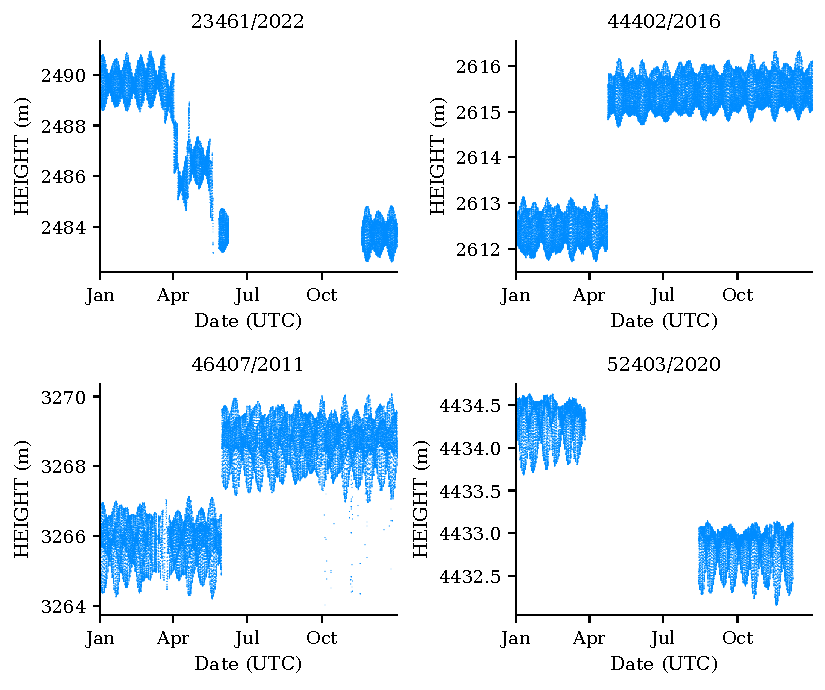
\includegraphics[width=\linewidth,height=0.81\textheight,keepaspectratio]{figures/presentation/full_record_context.pdf}
\caption{T=1 HEIGHT in meters for the four original records, with station and year labels. Points show the HEIGHT values, with blank intervals where observations are missing. The 44402 and 46407 steps occur near National Centers for Environmental Information (NCEI) deployment dates cited in Appendix~\ref{sec:scope}. At 52403, levels differ before and after a missing interval from March to August that includes the listed deployment date of 13 August 2020. The timing of that height change and the cause of the 23461 spikes remain unresolved. Figures~\ref{fig:dart_ecdf_fresh} and~\ref{fig:dart_spectra_fresh} give feature distributions and spectra for the three 2018 records.}
\label{fig:context}
\end{figure}

The encoder has hidden widths 128/64, rectified linear unit (ReLU) activations, and separate outputs for Gaussian means and log variances. Decoder hidden widths are 64/128, with ReLU activations and a linear residual output. Restricting log variance to $[-12,12]$ limits the variational family. Input clipping, a moving baseline, output smoothing, L2 penalties, and KL warmup are absent. Training uses Adam with batches of 64, learning rate $10^{-3}$, at most 10,000 steps, and a global gradient norm cap of 10. Original training windows are drawn uniformly with replacement; the 2018 records use UTC start hour weights. Training seeds are 42, 1729, and 31415, in that order in plots of individual fits. Within a seed, initial weights agree across conditions except for the residual output kernel and bias, which are multiplied by $b$ to preserve observation means. Each comparison uses fits with the same training seed.

For the original DART records, the training mean and standard deviation use every eligible training row once, including fragments too short to form a window. The scalar standard deviation has divisor $n$, the number of those rows. PPCA residual variance is the mean of the discarded covariance eigenvalues, subject to a positive minimum. For C, that minimum applies to the base variance before multiplication by $b^2$.

Original validation uses 64 importance samples per window and RNG stream 41001. Validation runs every 250 Adam steps; training stops after eight consecutive checks without improvement and retains the weights with the best validation estimate. Primary evaluation uses stream 42001. A sensitivity check with 1,024 samples uses 42002, and a separate repeat with 256 samples uses 42003. Prior samples use stream 43001. Final network weights are retained separately from the weights chosen by validation. All four conditions use this stopping rule; the iteration chosen by validation and the total number of steps can differ between fits.

\subsection{Additional DART records from 2018}
The additional cases use the calendar interval $[2018\text{-}01\text{-}01,2019\text{-}01\text{-}01)$, split 219 and 292 days after its start, with two days omitted on each side of both dates. Windows start at 00:00, 04:00, 08:00, 12:00, 16:00, or 20:00 UTC and require 192 consecutive source rows of finite T=1 HEIGHT values at most 9000, with unambiguous timestamps spaced 900 s apart. Any interruption ends a usable sequence. An eligible interval must span at least 240 days and contain valid routine observations in at least 80\% of its expected UTC slots at 15 minute spacing. Each partition must contain windows from all six start hours. Each partition must provide windows that share no source observations: at least 60 for training, 20 for validation, and 20 for testing. The corresponding train/validation/test counts are 101/33/33 for 44402, 104/32/23 for 21415, and 87/32/22 for 21418. Fitting and evaluation use the larger overlapping sets in Table~\ref{tab:data}. The calendar split determines the time intervals; these window counts measure the amount of usable data.

Within each partition, a window starting in UTC hour $j$ receives weight $1/(6n_j)$, where $n_j$ is the number of eligible starts in that hour. Each hour contributes one sixth of the weight to neural sampling, baseline fitting, variance choice, validation, and evaluation. Normalization gives each unique training observation in an eligible window equal weight and uses a population standard deviation. The observation set differs from that used for the original records, and equal observation weights differ from the UTC start hour weights on training windows. A secondary evaluation assigns equal weight to windows using the same scores. The data contain the eligible source measurements, without interpolation or augmentation. Equal weights for UTC start hours balance the clock times; tidal phases also depend on date and constituent frequency.

The choice of the 44402 annual case followed its examination and preceded this extension. The search excluded the four original stations and required listed coverage of all of 2018. The remaining stations were examined in identifier order. The first two annual records to meet the data requirements above were 21415 and 21418. Both entered the study before their neural model results were available. All 36 fits remain in the analysis. The catalogues document deployment periods \citep{NCEIDART44402,NCEIDART21415,NCEIDART21418}. Deployment dates alone leave hardware continuity uncertain.

The skip also lowers mean energy scores on all three additional cases in two separate checks: one uses network weights chosen by validation, and the other gives all windows equal weight. Comparing these cases with the original records also changes calendar splits, normalization data, evaluation stride, training duration, and weight selection. Attributing the different outcomes to deployment history would require separating these other changes.

For each additional record, PPCA fits use at most 16 loading directions and the training weights at variances $10^{-4},5\times10^{-4},2.5\times10^{-3},1.25\times10^{-2},6.25\times10^{-2}$. Exact weighted validation log density determines the variance, with larger variance winning an exact tie. All three records give the smallest grid value, $10^{-4}$, before neural fitting. The grid remains independent of test results. Each neural fit completes 10,000 Adam steps. Energy score on full validation windows is evaluated every 1,000 Adam steps using 512 prior samples and the validation window weights. The network weights with the lowest score are retained as a secondary set; ties retain the earlier weights. Conditions within each seed share training hyperparameters and initial observation means. Adam steps and gradient clipping use residual coordinates, so conditions can follow different training paths.

\begin{table}[H]
\centering
\setlength{\tabcolsep}{3pt}
\caption{Window counts and normalization constants. DART labels give the station and year of each routine T=1 record. Mean and scale are the training mean and population standard deviation in meters. For the original DART records, normalization uses every retained training row; for the 2018 records, it uses unique training rows in eligible windows. Gaussian observations retain their original coordinates, represented by mean zero and scale one. Base variance $\sigma_0^2$ is in squared model units; PPCA validation determines the 2018 values before neural fitting.}
\label{tab:data}
\begin{tabular}{lrrrrrr}
\toprule
Case & Train & Validation & Test & Mean & Scale & $\sigma_0^2$\\
\midrule
Gaussian & 8192 & 2048 & 2048 & 0 & 1 & 0.06157 \\
23461/2022 & 544 & 13 & 17 & 2488.8962 & 1.481 & 0.0001 \\
44402/2016 & 1153 & 34 & 35 & 2613.8301 & 1.518 & 0.0001 \\
46407/2011 & 983 & 26 & 27 & 3266.7902 & 1.48 & 0.0001 \\
52403/2020 & 339 & 17 & 16 & 4433.8446 & 0.7036 & 0.0001
\\
\midrule
44402/2018 & 1150 & 390 & 369 & 2615.7276 & 0.33 & 0.0001 \\
21415/2018 & 1227 & 364 & 215 & 4798.7832 & 0.3153 & 0.0001 \\
21418/2018 & 895 & 378 & 189 & 5726.9972 & 0.2634 & 0.0001
\\
\bottomrule
\end{tabular}
\end{table}

\section{ELBO terms and Gaussian baselines}
For Gaussian A/B, mean negative conditional log likelihood (NLL), averaged over posterior samples, rises from 0.04692 to 1.17735 nats per coordinate. This increase exceeds the decrease in analytic KL from 0.09338 to 0.02497 nats per coordinate. B and D also differ at the same observation variance: D's negative IW estimate ranges from 1.202 to 1.252 nats per coordinate. Encoder KL measures divergence from the prior. Reassignment tests how reconstruction depends on the encoder means assigned to windows. For one D seed, encoder KL to the prior is about $0.0003$ nats per window, compared with B's 4.81. Reassigning encoder means changes MSE in observation coordinates by zero at the recorded precision for that D fit, versus 0.405 and 0.453 for the other two.

For 46407 in 2011, mean NLL over posterior samples decreases from 27.0860 in A to $-0.6335$ in B, even as mean posterior expected MSE rises from 0.006154 to 0.007217 in squared standardized units. Equation~\ref{eq:elbo_components} explains these opposite orderings through density normalization and division of error by variance. Decoding the encoder mean also gives higher MSE in observation coordinates for B in two of the three comparisons by training seed.

The component analysis covers all 60 original models at their weights chosen by validation. The DART extension evaluates those 48 original DART models and 36 final models from 2018, keeping the original Gaussian analysis. The sampled terms use three independent streams, each with 256 posterior samples per test window. Conditional log likelihood, sampled $\log q-\log p(z)$, and importance weights use the same samples. Encoder KL to the prior is calculated analytically. Table~\ref{tab:components} averages test windows using each record's weights, then three sampling streams, then three training seeds. Reconstruction from the encoder mean and analytic KL depend only on the inputs and network weights. Negative ELBO uses analytic KL, whereas the Jensen difference uses sampled log ratios. Exact marginal log density remains unknown.

\clearpage
\begin{table}[H]
\centering
\setlength{\tabcolsep}{1.8pt}
\caption{Components at original observation variance. Original records use network weights chosen by validation and equal window weights; 2018 records use final network weights and UTC start hour weights. Raw MSE includes the input skip. Dividing by $b^2$ gives error in observation coordinates after decoding the encoder mean. For the 2018 fits, raw MSE is $b^2$ times this error; the original fits use the MSE saved during evaluation. Expected MSE and conditional negative log likelihood (NLL) are averaged over samples from $q_\phi(z\mid x)$. MSE uses squared model coordinates, and log quantities use nats per coordinate. Entries average test windows using their specified weights, then three sampling streams, then three fits. NLL and analytic KL sum to negative ELBO before rounding. IW is a separate estimate at finite $K$. A/C use $\sigma_0^2$, B/D use $25\sigma_0^2$; A/D have $\alpha=0$, B/C have $\alpha=0.8$.}
\label{tab:components}
\begin{tabular}{llrrrrrrr}
\toprule
Case & Condition & \shortstack{Raw\\MSE} & \shortstack{MSE\\$ / b^2$} & \shortstack{Expected\\MSE} & NLL/$d$ & KL/$d$ & \shortstack{Negative\\ELBO/$d$} & \shortstack{Negative\\IW/$d$}\\
\midrule
Gaussian & A & 0.0616 & 0.0616 & 0.06425 & 0.04692 & 0.09338 & 0.1403 & 0.1332 \\
Gaussian & B & 0.003683 & 0.09209 & 0.1316 & 1.177 & 0.02497 & 1.202 & 1.201 \\
Gaussian & C & 0.002496 & 0.06239 & 0.06498 & 0.05287 & 0.09343 & 0.1463 & 0.1373 \\
Gaussian & D & 0.1985 & 0.1985 & 0.2182 & 1.205 & 0.01483 & 1.22 & 1.22 \\
23461/2022 & A & 0.0008939 & 0.0008939 & 0.0008945 & 0.7864 & 1.447 & 2.233 & 2.065 \\
23461/2022 & B & \ensuremath{8.379\times10^{-5}} & 0.002095 & 0.002121 & -1.653 & 0.5324 & -1.12 & -1.228 \\
23461/2022 & C & 0.000102 & 0.002551 & 0.002552 & 9.073 & 1.372 & 10.44 & 10.06 \\
23461/2022 & D & 0.001201 & 0.001201 & 0.001207 & -1.835 & 0.6391 & -1.196 & -1.234 \\
44402/2016 & A & 0.0003423 & 0.0003423 & 0.0003479 & -1.947 & 0.5698 & -1.377 & -1.573 \\
44402/2016 & B & \ensuremath{1.723\times10^{-5}} & 0.0004308 & 0.0004851 & -1.98 & 0.1266 & -1.853 & -1.894 \\
44402/2016 & C & \ensuremath{1.509\times10^{-5}} & 0.0003771 & 0.0003828 & -1.772 & 0.5071 & -1.265 & -1.58 \\
44402/2016 & D & 0.0003269 & 0.0003269 & 0.0003903 & -1.999 & 0.1313 & -1.867 & -1.89 \\
46407/2011 & A & 0.006143 & 0.006143 & 0.006154 & 27.09 & 0.553 & 27.64 & 27 \\
46407/2011 & B & 0.0002783 & 0.006957 & 0.007217 & -0.6335 & 0.2009 & -0.4326 & -0.6198 \\
46407/2011 & C & 0.000274 & 0.00685 & 0.006867 & 30.65 & 0.5804 & 31.23 & 30.12 \\
46407/2011 & D & 0.006611 & 0.006611 & 0.006824 & -0.712 & 0.2272 & -0.4848 & -0.6253 \\
52403/2020 & A & 0.0009731 & 0.0009731 & 0.0009804 & 1.216 & 0.5951 & 1.811 & 1.38 \\
52403/2020 & B & \ensuremath{9.723\times10^{-5}} & 0.002431 & 0.002613 & -1.554 & 0.2245 & -1.33 & -1.533 \\
52403/2020 & C & \ensuremath{7.928\times10^{-5}} & 0.001982 & 0.00199 & 6.265 & 0.5363 & 6.801 & 5.821 \\
52403/2020 & D & 0.001278 & 0.001278 & 0.001487 & -1.779 & 0.1976 & -1.582 & -1.686 \\
44402/2018 & A & 0.001983 & 0.001983 & 0.001987 & 6.247 & 0.5841 & 6.831 & 6.402 \\
44402/2018 & B & 0.0001297 & 0.003242 & 0.003332 & -1.41 & 0.3115 & -1.099 & -1.253 \\
44402/2018 & C & 0.0001096 & 0.00274 & 0.002743 & 10.03 & 0.5617 & 10.59 & 10.05 \\
44402/2018 & D & 0.002506 & 0.002506 & 0.002634 & -1.55 & 0.2993 & -1.251 & -1.383 \\
21415/2018 & A & 0.001018 & 0.001018 & 0.001021 & 1.421 & 0.6215 & 2.042 & 1.753 \\
21415/2018 & B & 0.0001031 & 0.002576 & 0.002735 & -1.53 & 0.286 & -1.244 & -1.418 \\
21415/2018 & C & \ensuremath{9.305\times10^{-5}} & 0.002326 & 0.002329 & 7.961 & 0.5846 & 8.546 & 8.018 \\
21415/2018 & D & 0.001274 & 0.001274 & 0.001435 & -1.79 & 0.2931 & -1.497 & -1.61 \\
21418/2018 & A & 0.001534 & 0.001534 & 0.001544 & 4.031 & 0.6301 & 4.661 & 4.16 \\
21418/2018 & B & 0.0001342 & 0.003355 & 0.003529 & -1.371 & 0.2885 & -1.082 & -1.292 \\
21418/2018 & C & 0.0001236 & 0.00309 & 0.0031 & 11.81 & 0.5499 & 12.36 & 11.33 \\
21418/2018 & D & 0.001673 & 0.001673 & 0.001863 & -1.704 & 0.2886 & -1.416 & -1.54
\\
\bottomrule
\end{tabular}
\end{table}

\begin{table}[H]
\centering
\caption{Gaussian baseline scores over test realizations. Lower is better. Exact negative log densities use nats per coordinate; energy score uses the original dimensionless Gaussian coordinates. Each baseline uses 512 standard normal samples transformed by its covariance Cholesky factor. True Gaussian is the known generating density. DART baselines use the separate evaluation with three streams in Table~\ref{tab:dart_energy}.}
\begin{tabular}{llrr}
\toprule
Case & Model & Negative log score & Energy score\\
\midrule
Gaussian & True Gaussian & 0.1255 & 5.717 \\
Gaussian & PPCA & 0.1266 & 5.72 \\
Gaussian & Diagonal Gaussian & 0.9087 & 5.793 \\
\\
\bottomrule
\end{tabular}
\end{table}

Proposition~\ref{prop:equivalence} holds in exact arithmetic. With single precision arithmetic, applying the map to all \PrigmJobCount{} original fits gave maximum absolute differences of \PrigmMaxMappedLogDensityError{} nat in conditional log density and \PrigmMaxMappedSampleMeanError{} in conditional means, in model coordinates. The 1 nat difference occurs for a C to A map on DART at a large absolute log density, under relative tolerance $3\times10^{-5}$ and absolute tolerance 0.01 nats. Gaussian differences stay below $2\times10^{-4}$ nats. This check uses the first eight validation windows and prior latent samples. Marginal IW estimates use a different calculation on the full test set with different encoder samples. The conditional density check leaves the accuracy of marginal IW estimates unresolved. In a separate sampling check, the largest absolute change in a fit's mean IW estimate on the initial test subset between 256 and 1,024 samples was \PrigmMaxAbsStabilityScoreChange{} nats per coordinate.

\begingroup
\setlength{\tabcolsep}{3pt}
\begin{longtable}{llrrrrrrrr}
\caption{All 12 original Gaussian fits. Raw MSE decodes the encoder mean with the input skip; division by $b^2$ gives error in observation coordinates. Both use squared dimensionless coordinates. Negative IW is estimated negative log density in nats per coordinate, and KL uses nats per realization. Energy score uses 512 prior samples per fit. For each fit, errors, KL, and energy score are averaged over all test realizations. Lower errors and scores are preferable; KL measures encoder divergence. ESS is calculated from 256 importance samples for each realization. The table reports its median across realizations. Step gives the Adam iteration chosen by validation. A/C use $\sigma_0^2$, B/D use $25\sigma_0^2$; A/D have $\alpha=0$, B/C have $\alpha=0.8$.}\\
\toprule
Case & Condition & Seed & Step & \shortstack{Raw\\MSE} & MSE/$b^2$ & \shortstack{Negative\\IW} & KL & \shortstack{Energy\\score} & ESS\\
\midrule
\endfirsthead
\toprule
Case & Condition & Seed & Step & \shortstack{Raw\\MSE} & MSE/$b^2$ & \shortstack{Negative\\IW} & KL & \shortstack{Energy\\score} & ESS\\
\midrule
\endhead
Gaussian & A & 42 & 5000 & 0.06162 & 0.06162 & 0.1335 & 17.94 & 5.723 & 41.3 \\
Gaussian & A & 1729 & 5250 & 0.0617 & 0.0617 & 0.1334 & 18.06 & 5.724 & 35.68 \\
Gaussian & A & 31415 & 7750 & 0.06149 & 0.06149 & 0.1326 & 17.79 & 5.721 & 52.9 \\
Gaussian & B & 42 & 10000 & 0.003662 & 0.09155 & 1.201 & 4.814 & 7.13 & 202.3 \\
Gaussian & B & 1729 & 5750 & 0.003704 & 0.09261 & 1.201 & 4.78 & 7.123 & 180.1 \\
Gaussian & B & 31415 & 8750 & 0.003684 & 0.0921 & 1.201 & 4.787 & 7.118 & 196.3 \\
Gaussian & C & 42 & 10000 & 0.002494 & 0.06236 & 0.1371 & 17.9 & 5.719 & 31.33 \\
Gaussian & C & 1729 & 6000 & 0.002497 & 0.06243 & 0.1376 & 17.96 & 5.722 & 29.33 \\
Gaussian & C & 31415 & 7500 & 0.002496 & 0.06239 & 0.1371 & 17.96 & 5.724 & 29.24 \\
Gaussian & D & 42 & 750 & 0.3608 & 0.3608 & 1.252 & 0.0003156 & 6.901 & 255.8 \\
Gaussian & D & 1729 & 5500 & 0.1306 & 0.1306 & 1.205 & 3.881 & 7.088 & 209.9 \\
Gaussian & D & 31415 & 6250 & 0.1042 & 0.1042 & 1.202 & 4.658 & 7.118 & 206.5 \\
\\
\bottomrule
\end{longtable}
\endgroup

\subsection{Importance weighted log density}
\begin{table}[H]
\centering
\caption{Original differences in estimated negative IW log density at $K=256$, in nats per coordinate. Each difference compares fits with the same training seed. Cells give the median across three seeds and the full range underneath. Negative values favor the first condition. DART labels give station and year for the original records. These finite importance estimates leave rankings by exact marginal likelihood uncertain. A/C share $\sigma_0^2$ and B/D share $25\sigma_0^2$; A/B also changes variance.}
\label{tab:results}
\begin{tabular}{lccc}
\toprule
Case & $B{-}A$ & $C{-}A$ & $B{-}D$\\
\midrule
Gaussian & \shortstack{$1.068$\\$[1.068,\,1.069]$} & \shortstack{$0.004143$\\$[0.003679,\,0.004428]$} & \shortstack{$-0.004057$\\$[-0.05053,\,-0.0009969]$} \\
23461/2022 & \shortstack{$-4.328$\\$[-4.52,\,-1.029]$} & \shortstack{$9.496$\\$[3.226,\,11.24]$} & \shortstack{$-0.02887$\\$[-0.2702,\,0.3098]$} \\
44402/2016 & \shortstack{$-0.3495$\\$[-0.4308,\,-0.1869]$} & \shortstack{$-0.1457$\\$[-0.7499,\,0.8596]$} & \shortstack{$-0.002817$\\$[-0.007894,\,0.00181]$} \\
46407/2011 & \shortstack{$-26.65$\\$[-30.07,\,-26.16]$} & \shortstack{$2.374$\\$[2.168,\,4.924]$} & \shortstack{$-0.01531$\\$[-0.02908,\,0.0532]$} \\
52403/2020 & \shortstack{$-2.595$\\$[-3.644,\,-2.527]$} & \shortstack{$4.26$\\$[3.937,\,5.114]$} & \shortstack{$0.1918$\\$[0.05503,\,0.2004]$}
\\
\bottomrule
\end{tabular}
\end{table}

Low initial DART effective sample sizes prompted evaluation with 4,096 and 16,384 samples using two additional sampling streams and the same network weights. Each sample count uses the first 32 test windows, or all windows when fewer are available: 32 Gaussian, 17 from 23461, 32 from 44402, 27 from 46407, and 16 from 52403. Table~\ref{tab:refinement} compares those windows with their original estimates at 256 samples. The Gaussian and 44402 subsets are smaller than the full test sets in the main results.

Even with more samples, the accuracy of the marginal log density estimate remains unknown. Between 256 and 16,384 samples, the largest absolute change in a fit's mean estimate was 0.468 nats per coordinate on DART and 0.000868 on Gaussian data. At 16,384 samples, median DART ESS per fit ranged from 1.0001 to 23.4. C's negative IW estimate exceeds A's for 23461, 46407, and 52403 at every sample count and encoder distribution tested. The direction for 44402 varies by training seed. B/D differences take both signs for 23461, 44402, and 46407; on 52403, B's estimate exceeds D's at every seed and sample count tested.

\begin{table}[H]
\centering
\setlength{\tabcolsep}{1.4pt}
\caption{Importance estimates with more samples on the same initial test windows. DART labels give station and year. Differences compare conditions with the same training seed. Cells give the median difference in negative IW log density, in nats per coordinate, and the full range across three seeds underneath. Negative values favor the first condition. The Gaussian and 44402 subsets are smaller than their full test sets. A/C use $\sigma_0^2$, B/D use $25\sigma_0^2$; A/D have $\alpha=0$, B/C have $\alpha=0.8$.}
\label{tab:refinement}
\begin{tabular}{llccc}
\toprule
Case & $\Delta$ & $K=256$ & $K=4096$ & $K=16384$\\
\midrule
Gaussian & $B-A$ & \shortstack{$1.068$\\$[1.068,\,1.069]$} & \shortstack{$1.069$\\$[1.069,\,1.069]$} & \shortstack{$1.069$\\$[1.069,\,1.069]$} \\
Gaussian & $C-A$ & \shortstack{$0.003605$\\$[0.001233,\,0.004018]$} & \shortstack{$0.003406$\\$[0.001593,\,0.00391]$} & \shortstack{$0.003707$\\$[0.001884,\,0.00389]$} \\
Gaussian & $B-D$ & \shortstack{$-0.00525$\\$[-0.05736,\,\ensuremath{9.69\times10^{-5}}]$} & \shortstack{$-0.005248$\\$[-0.05733,\,\ensuremath{9.666\times10^{-5}}]$} & \shortstack{$-0.005238$\\$[-0.05736,\,0.000105]$} \\
23461/2022 & $B-A$ & \shortstack{$-4.328$\\$[-4.52,\,-1.029]$} & \shortstack{$-4.286$\\$[-4.527,\,-1.026]$} & \shortstack{$-4.262$\\$[-4.502,\,-1.011]$} \\
23461/2022 & $C-A$ & \shortstack{$9.496$\\$[3.226,\,11.24]$} & \shortstack{$9.462$\\$[3.209,\,11.11]$} & \shortstack{$9.455$\\$[3.185,\,11.05]$} \\
23461/2022 & $B-D$ & \shortstack{$-0.02887$\\$[-0.2702,\,0.3098]$} & \shortstack{$-0.03072$\\$[-0.3078,\,0.302]$} & \shortstack{$-0.02819$\\$[-0.3055,\,0.3093]$} \\
44402/2016 & $B-A$ & \shortstack{$-0.2881$\\$[-0.3638,\,-0.1447]$} & \shortstack{$-0.2255$\\$[-0.3328,\,-0.1409]$} & \shortstack{$-0.1959$\\$[-0.3169,\,-0.1381]$} \\
44402/2016 & $C-A$ & \shortstack{$-0.1264$\\$[-0.7203,\,0.8996]$} & \shortstack{$-0.1789$\\$[-0.7328,\,0.8346]$} & \shortstack{$-0.1953$\\$[-0.7254,\,0.807]$} \\
44402/2016 & $B-D$ & \shortstack{$-0.00224$\\$[-0.009321,\,0.002505]$} & \shortstack{$-0.01095$\\$[-0.01247,\,0.002069]$} & \shortstack{$-0.01189$\\$[-0.01382,\,0.0006799]$} \\
46407/2011 & $B-A$ & \shortstack{$-26.65$\\$[-30.07,\,-26.16]$} & \shortstack{$-26.54$\\$[-29.86,\,-26.04]$} & \shortstack{$-26.48$\\$[-29.81,\,-25.97]$} \\
46407/2011 & $C-A$ & \shortstack{$2.374$\\$[2.168,\,4.924]$} & \shortstack{$2.281$\\$[2.09,\,4.798]$} & \shortstack{$2.275$\\$[2.011,\,4.8]$} \\
46407/2011 & $B-D$ & \shortstack{$-0.01531$\\$[-0.02908,\,0.0532]$} & \shortstack{$-0.02418$\\$[-0.03144,\,0.04631]$} & \shortstack{$-0.03034$\\$[-0.03092,\,0.04173]$} \\
52403/2020 & $B-A$ & \shortstack{$-2.595$\\$[-3.644,\,-2.527]$} & \shortstack{$-2.555$\\$[-3.565,\,-2.497]$} & \shortstack{$-2.521$\\$[-3.523,\,-2.462]$} \\
52403/2020 & $C-A$ & \shortstack{$4.26$\\$[3.937,\,5.114]$} & \shortstack{$4.112$\\$[3.735,\,4.988]$} & \shortstack{$4.139$\\$[3.595,\,4.974]$} \\
52403/2020 & $B-D$ & \shortstack{$0.1918$\\$[0.05503,\,0.2004]$} & \shortstack{$0.168$\\$[0.031,\,0.1719]$} & \shortstack{$0.1566$\\$[0.0255,\,0.1715]$}
\\
\bottomrule
\end{tabular}
\end{table}

\section{Window means, shape, and energy scores}
With each record's weights, the variance across all window entries equals the mean variance within windows plus the variance of window means. The first accounts for 4.80 to 16.69\% of training variance across the original records, 99.14 to 99.68\% of their later test variance, and 95.99 to 99.32\% of training variance across the three additional records. Each range uses the weights for that record and partition. The two variance terms add directly. In energy score, mean and shape differences enter the same Euclidean norm, so their score contributions are inseparable by this variance decomposition. At 44402, the 2016 height step occurs near the listed deployment date of 23 April, while the 2018 record lies within one listed deployment. The cause of the height step remains uncertain despite its proximity to the deployment date.

Let $P x=x-\bar x\mathbf 1$ subtract a window's own mean, for both observations and generated samples. The energy scores use full windows $x$, windows after mean subtraction $Px$, and the vector of time increments
\begin{equation}
\Phi(x)=\left(\frac{x_{t+\ell}-x_t}{\sqrt{192-\ell}}\right)_{\ell\in\mathcal L,\;0\leq t<192-\ell},
\qquad \mathcal L=\{1,4,16,48,96\}.
\label{eq:increments}
\end{equation}
The vector of time increments has 795 coordinates. Since it includes adjacent differences, $\ker\Phi=\operatorname{span}\{\mathbf 1\}$ and $\operatorname{rank}\Phi=191$. It determines window shape up to an additive constant, including dependence across positions. Extra lags change the distance: writing $\Phi(x)=Ax$ gives $\sqrt{(x-y)^\top A^\top A(x-y)}$, in place of Euclidean distance between $Px$ and $Py$. Under finite first moments, the energy scores of $Px$ and $\Phi(x)$ are proper for their respective distributions. Both operations remove window means. Their scores therefore assess the resulting shape distributions; the score on full windows also assesses mean levels and their dependence on shape. The two shape scores use different distances.

All DART scores use standardized coordinates. Conversion to meters would multiply energy scores by the positive training scale for each record. Three independent prior streams each draw 1,024 latent values and standard normal noise vectors. Each condition scales the noise by its own observation standard deviation. Within each record, comparisons across conditions and between original and estimated observation variances use the same latent values and standard normal noise samples. IW uses three separate posterior streams. For each fit, summaries first average the three sampling streams. Condition differences compare the same training seed and sampling stream. Ranges across training seeds describe differences among fitted models. Repeated sampling within a fit measures Monte Carlo variation.

\begingroup
\setlength{\tabcolsep}{2.4pt}
\begin{longtable}{lllrrr}
\caption{DART energy score differences at the same observation variance, in standardized coordinates. Scores use full windows, windows after subtraction of their own means, or time increments from Eq.~\ref{eq:increments}. Negative values favor the skip. C-A uses $\sigma_0^2$ and B-D uses $25\sigma_0^2$. Seed rows give the median across three training seeds and the full range underneath, comparing conditions with the same seed. Monte Carlo width gives the largest range, within a seed, of differences from the three common sampling streams. Original records use network weights chosen by validation and equal window weights; 2018 cases use final network weights and equal total window weight in each UTC start hour.}\label{tab:dart_contrasts}\\
\toprule
Record & $\Delta$ & Summary & \shortstack{Full\\windows} & \shortstack{After mean\\subtraction} & \shortstack{Time\\increments}\\
\midrule
\endfirsthead
\toprule
Record & $\Delta$ & Summary & \shortstack{Full\\windows} & \shortstack{After mean\\subtraction} & \shortstack{Time\\increments}\\
\midrule
\endhead
23461/2022 & C-A & Seed & \shortstack{0.369\\{[-1.21, 1.5]}} & \shortstack{0.0255\\{[-0.0553, 0.297]}} & \shortstack{0.00303\\{[-0.00289, 0.0262]}} \\
23461/2022 & C-A & Monte Carlo width & 0.1585 & 0.03316 & 0.004819 \\
23461/2022 & B-D & Seed & \shortstack{0.83\\{[0.773, 3.4]}} & \shortstack{0.0822\\{[-0.0275, 0.0868]}} & \shortstack{0.0111\\{[0.000783, 0.0154]}} \\
23461/2022 & B-D & Monte Carlo width & 0.4628 & 0.03795 & 0.005022 \\
44402/2016 & C-A & Seed & \shortstack{-0.153\\{[-1.27, 0.849]}} & \shortstack{-0.0814\\{[-0.144, 0.032]}} & \shortstack{-0.00857\\{[-0.0311, 0.0141]}} \\
44402/2016 & C-A & Monte Carlo width & 0.2093 & 0.02672 & 0.004928 \\
44402/2016 & B-D & Seed & \shortstack{0.115\\{[0.111, 0.172]}} & \shortstack{0.0313\\{[0.0256, 0.0371]}} & \shortstack{0.00319\\{[0.000627, 0.00757]}} \\
44402/2016 & B-D & Monte Carlo width & 0.4656 & 0.05392 & 0.006256 \\
46407/2011 & C-A & Seed & \shortstack{0.903\\{[-0.887, 0.936]}} & \shortstack{-0.0851\\{[-0.0892, -0.0797]}} & \shortstack{-0.00199\\{[-0.00548, -0.000733]}} \\
46407/2011 & C-A & Monte Carlo width & 0.1399 & 0.04674 & 0.006484 \\
46407/2011 & B-D & Seed & \shortstack{0.103\\{[-0.327, 0.111]}} & \shortstack{-0.0148\\{[-0.0668, 0.0736]}} & \shortstack{-0.000348\\{[-0.00275, 0.0147]}} \\
46407/2011 & B-D & Monte Carlo width & 0.2988 & 0.0161 & 0.002748 \\
52403/2020 & C-A & Seed & \shortstack{-0.407\\{[-0.836, 0.753]}} & \shortstack{-0.0297\\{[-0.0601, 0.0404]}} & \shortstack{-0.00367\\{[-0.00459, 0.0071]}} \\
52403/2020 & C-A & Monte Carlo width & 0.1334 & 0.03162 & 0.004903 \\
52403/2020 & B-D & Seed & \shortstack{1.18\\{[-0.604, 3.18]}} & \shortstack{-0.0156\\{[-0.0214, -0.0122]}} & \shortstack{-0.00419\\{[-0.00425, -0.00196]}} \\
52403/2020 & B-D & Monte Carlo width & 0.3057 & 0.05334 & 0.008483 \\
44402/2018 & C-A & Seed & \shortstack{-0.337\\{[-0.768, -0.119]}} & \shortstack{-0.345\\{[-0.479, -0.296]}} & \shortstack{-0.035\\{[-0.0523, -0.0334]}} \\
44402/2018 & C-A & Monte Carlo width & 0.05621 & 0.04827 & 0.007899 \\
44402/2018 & B-D & Seed & \shortstack{-0.222\\{[-0.322, -0.219]}} & \shortstack{-0.228\\{[-0.363, -0.151]}} & \shortstack{-0.0268\\{[-0.042, -0.0156]}} \\
44402/2018 & B-D & Monte Carlo width & 0.06129 & 0.04827 & 0.006903 \\
21415/2018 & C-A & Seed & \shortstack{-0.3\\{[-0.346, -0.227]}} & \shortstack{-0.372\\{[-0.393, -0.327]}} & \shortstack{-0.0564\\{[-0.058, -0.0467]}} \\
21415/2018 & C-A & Monte Carlo width & 0.02322 & 0.02964 & 0.004697 \\
21415/2018 & B-D & Seed & \shortstack{-0.253\\{[-0.341, -0.236]}} & \shortstack{-0.252\\{[-0.32, -0.223]}} & \shortstack{-0.0375\\{[-0.051, -0.0349]}} \\
21415/2018 & B-D & Monte Carlo width & 0.06139 & 0.0564 & 0.009434 \\
21418/2018 & C-A & Seed & \shortstack{-0.613\\{[-0.852, -0.266]}} & \shortstack{-0.453\\{[-0.626, -0.411]}} & \shortstack{-0.0577\\{[-0.0901, -0.0548]}} \\
21418/2018 & C-A & Monte Carlo width & 0.05868 & 0.02613 & 0.003922 \\
21418/2018 & B-D & Seed & \shortstack{-0.476\\{[-0.559, -0.433]}} & \shortstack{-0.501\\{[-0.544, -0.357]}} & \shortstack{-0.0685\\{[-0.074, -0.0524]}} \\
21418/2018 & B-D & Monte Carlo width & 0.03753 & 0.05253 & 0.008115
\\
\bottomrule
\end{longtable}
\endgroup

\subsection{Baseline distributions}
\label{sec:reference_distributions}
Baseline fits use the mean and covariance of training windows, with equal window weights for the original records and equal total weight in each UTC start hour for 2018. With $v=\sigma_0^2$, PPCA at the neural observation variance has covariance $WW^\top+vI$ or $WW^\top+25vI$. Its at most 16 loading directions follow leading covariance eigenvectors, with magnitudes $\sqrt{\max(\lambda_j-v,0)}$ at variance $v$. For the diagonal Gaussian, each coordinate variance is the larger of its empirical variance and the imposed noise variance. A separate PPCA fit estimates noise as the average discarded eigenvalue, subject to a minimum of $10^{-4}$. It gives $10^{-4}$ for the original records and 21415/2018, approximately $1.10338\times10^{-4}$ for 21418/2018, and $1.20477\times10^{-4}$ for 44402/2018. When the noise estimate equals the neural observation variance, the two PPCA fits define the same distribution.

Each baseline is evaluated with three random sampling streams of 1,024 samples. Variation across streams measures sampling variation for that distribution. The baseline distributions stay the same during the neural variance replacement comparison. Table~\ref{tab:dart_energy} compares their energy scores with those of the neural fits.

PPCA has lower mean energy scores than every neural fit at the same observation variance, across all 84 fits and all three scores. Its lower scores after mean subtraction and on time increments show that this difference also concerns variation within windows. PPCA parameters come from covariance eigendecomposition \citep{TippingBishop1999ProbabilisticPCA}; neural fits use variational inference and a finite number of optimizer steps. The comparison combines differences in model class and fitting procedure. Energy scores compare unconditional prior samples with test observations. Posterior importance weights enter only the log density calculation.

The training covariance helps explain why a linear baseline is useful here. Let $S=\sum_j\lambda_j u_j u_j^\top$ be covariance about the mean window, using the training weights, with eigenvalues in decreasing order. For each scoring transform $T\in\{I,P,\Phi\}$, the fraction $\sum_{j=1}^{16}\lambda_j\|Tu_j\|^2/\operatorname{tr}(TST^\top)$ exceeds 99.97\% on every record. Thus the leading 16 directions account for almost all empirical covariance trace, including after mean subtraction and for time increments. Gaussianity, dependence beyond covariance, and convergence of neural training remain undetermined by this calculation.

\begingroup
\setlength{\tabcolsep}{3pt}
\begin{longtable}{llrrr}
\caption{DART energy scores in standardized coordinates. Lower is better. Scores use full windows, windows after subtraction of their own means, or time increments from Eq.~\ref{eq:increments}. Neural A--D rows give the median across three training seeds and the full range, after averaging three sampling streams per fit. Baseline rows give the mean and range across three streams from a single fit. PPCA fitted estimates noise variance; PPCA matched uses the neural observation variance. These ranges measure different sources of variation. A/C use $v=\sigma_0^2$, B/D use $25v$; A/D have $\alpha=0$, B/C have $\alpha=0.8$. Original cases use network weights chosen by validation and equal window weights; 2018 cases use final network weights and UTC start hour weights.}\label{tab:dart_energy}\\
\toprule
Record & Model & \shortstack{Full\\windows} & \shortstack{After mean\\subtraction} & \shortstack{Time\\increments}\\
\midrule
\endfirsthead
\toprule
Record & Model & \shortstack{Full\\windows} & \shortstack{After mean\\subtraction} & \shortstack{Time\\increments}\\
\midrule
\endhead
23461/2022 & A & 45.3 [44.1, 45.5] & 3.27 [3.18, 3.35] & 0.437 [0.434, 0.457] \\
23461/2022 & B & 46.1 [44.8, 47.1] & 3.21 [3.14, 3.29] & 0.426 [0.421, 0.439] \\
23461/2022 & C & 44.5 [44.3, 46.8] & 3.22 [3.21, 3.65] & 0.437 [0.434, 0.483] \\
23461/2022 & D & 44 [43.7, 45.2] & 3.17 [3.12, 3.21] & 0.421 [0.411, 0.428] \\
23461/2022 & PPCA fitted & 42.1 [41.9, 42.3] & 2.94 [2.93, 2.97] & 0.399 [0.397, 0.402] \\
23461/2022 & PPCA matched ($v$) & 42.1 [41.9, 42.3] & 2.94 [2.93, 2.97] & 0.399 [0.397, 0.402] \\
23461/2022 & Diagonal ($v$) & 42.5 [42.5, 42.6] & 4.56 [4.56, 4.57] & 0.934 [0.932, 0.935] \\
23461/2022 & PPCA matched ($25v$) & 42.2 [42, 42.5] & 2.95 [2.94, 2.96] & 0.4 [0.399, 0.401] \\
23461/2022 & Diagonal ($25v$) & 42.5 [42.5, 42.6] & 4.56 [4.56, 4.57] & 0.934 [0.932, 0.935] \\
44402/2016 & A & 12.6 [12.2, 13.6] & 2.25 [2.22, 2.32] & 0.309 [0.308, 0.326] \\
44402/2016 & B & 11.6 [11.3, 12.2] & 2.07 [2.06, 2.09] & 0.278 [0.277, 0.283] \\
44402/2016 & C & 13.4 [10.9, 13.4] & 2.18 [2.16, 2.25] & 0.3 [0.295, 0.322] \\
44402/2016 & D & 11.5 [11.2, 12] & 2.04 [2.04, 2.05] & 0.276 [0.275, 0.276] \\
44402/2016 & PPCA fitted & 9.06 [8.94, 9.21] & 1.97 [1.95, 1.98] & 0.268 [0.266, 0.27] \\
44402/2016 & PPCA matched ($v$) & 9.06 [8.94, 9.21] & 1.97 [1.95, 1.98] & 0.268 [0.266, 0.27] \\
44402/2016 & Diagonal ($v$) & 10.4 [10.4, 10.5] & 4.37 [4.36, 4.37] & 0.952 [0.95, 0.953] \\
44402/2016 & PPCA matched ($25v$) & 9.04 [8.94, 9.19] & 1.97 [1.96, 1.98] & 0.269 [0.267, 0.269] \\
44402/2016 & Diagonal ($25v$) & 10.4 [10.4, 10.5] & 4.37 [4.36, 4.37] & 0.952 [0.95, 0.953] \\
46407/2011 & A & 15.5 [14.9, 16.1] & 4.79 [4.74, 4.8] & 0.676 [0.664, 0.677] \\
46407/2011 & B & 13.4 [13.4, 13.9] & 4.47 [4.39, 4.49] & 0.643 [0.633, 0.646] \\
46407/2011 & C & 16.5 [14, 17] & 4.71 [4.66, 4.71] & 0.672 [0.662, 0.675] \\
46407/2011 & D & 13.8 [13.3, 13.8] & 4.46 [4.39, 4.5] & 0.635 [0.629, 0.646] \\
46407/2011 & PPCA fitted & 12.6 [12.4, 12.8] & 4.13 [4.12, 4.14] & 0.601 [0.6, 0.603] \\
46407/2011 & PPCA matched ($v$) & 12.6 [12.4, 12.8] & 4.13 [4.12, 4.14] & 0.601 [0.6, 0.603] \\
46407/2011 & Diagonal ($v$) & 13.8 [13.8, 13.8] & 5.29 [5.28, 5.3] & 1.04 [1.04, 1.04] \\
46407/2011 & PPCA matched ($25v$) & 12.5 [12.5, 12.7] & 4.13 [4.12, 4.15] & 0.6 [0.598, 0.603] \\
46407/2011 & Diagonal ($25v$) & 13.8 [13.8, 13.8] & 5.29 [5.28, 5.3] & 1.04 [1.04, 1.04] \\
52403/2020 & A & 18.5 [18.3, 19.2] & 3.55 [3.5, 3.55] & 0.538 [0.534, 0.543] \\
52403/2020 & B & 15.9 [14.3, 18.2] & 3.37 [3.36, 3.39] & 0.518 [0.516, 0.523] \\
52403/2020 & C & 18.1 [17.5, 20] & 3.52 [3.49, 3.54] & 0.54 [0.534, 0.541] \\
52403/2020 & D & 14.9 [14.7, 15] & 3.39 [3.38, 3.4] & 0.522 [0.52, 0.525] \\
52403/2020 & PPCA fitted & 11 [10.9, 11.2] & 3.16 [3.11, 3.2] & 0.491 [0.483, 0.498] \\
52403/2020 & PPCA matched ($v$) & 11 [10.9, 11.2] & 3.16 [3.11, 3.2] & 0.491 [0.483, 0.498] \\
52403/2020 & Diagonal ($v$) & 12.3 [12.3, 12.3] & 5.03 [5.02, 5.04] & 1.06 [1.06, 1.07] \\
52403/2020 & PPCA matched ($25v$) & 11.1 [11, 11.2] & 3.15 [3.11, 3.17] & 0.488 [0.483, 0.492] \\
52403/2020 & Diagonal ($25v$) & 12.3 [12.3, 12.3] & 5.03 [5.02, 5.04] & 1.06 [1.06, 1.07] \\
44402/2018 & A & 12.4 [12.3, 12.5] & 12 [11.9, 12] & 1.58 [1.57, 1.59] \\
44402/2018 & B & 11.2 [11.2, 11.3] & 10.8 [10.8, 10.8] & 1.44 [1.44, 1.45] \\
44402/2018 & C & 12 [11.7, 12.3] & 11.6 [11.5, 11.7] & 1.54 [1.52, 1.55] \\
44402/2018 & D & 11.5 [11.4, 11.5] & 11.1 [11, 11.1] & 1.47 [1.46, 1.48] \\
44402/2018 & PPCA fitted & 9.8 [9.79, 9.81] & 9.41 [9.39, 9.42] & 1.27 [1.27, 1.27] \\
44402/2018 & PPCA matched ($v$) & 9.8 [9.79, 9.81] & 9.41 [9.39, 9.42] & 1.27 [1.27, 1.27] \\
44402/2018 & Diagonal ($v$) & 10.3 [10.3, 10.3] & 9.99 [9.99, 9.99] & 1.46 [1.46, 1.46] \\
44402/2018 & PPCA matched ($25v$) & 9.79 [9.79, 9.79] & 9.4 [9.39, 9.4] & 1.27 [1.27, 1.27] \\
44402/2018 & Diagonal ($25v$) & 10.3 [10.3, 10.3] & 9.99 [9.99, 9.99] & 1.46 [1.46, 1.46] \\
21415/2018 & A & 11.7 [11.6, 11.7] & 11.5 [11.4, 11.5] & 1.8 [1.79, 1.81] \\
21415/2018 & B & 10.6 [10.6, 10.7] & 10.4 [10.4, 10.5] & 1.63 [1.63, 1.65] \\
21415/2018 & C & 11.4 [11.3, 11.5] & 11.1 [11.1, 11.2] & 1.75 [1.74, 1.75] \\
21415/2018 & D & 10.9 [10.8, 11] & 10.7 [10.6, 10.7] & 1.68 [1.67, 1.68] \\
21415/2018 & PPCA fitted & 9.56 [9.55, 9.57] & 9.35 [9.34, 9.35] & 1.47 [1.47, 1.47] \\
21415/2018 & PPCA matched ($v$) & 9.56 [9.55, 9.57] & 9.35 [9.34, 9.35] & 1.47 [1.47, 1.47] \\
21415/2018 & Diagonal ($v$) & 9.92 [9.92, 9.93] & 9.74 [9.74, 9.75] & 1.61 [1.61, 1.61] \\
21415/2018 & PPCA matched ($25v$) & 9.56 [9.55, 9.56] & 9.35 [9.34, 9.35] & 1.47 [1.47, 1.47] \\
21415/2018 & Diagonal ($25v$) & 9.92 [9.92, 9.93] & 9.74 [9.74, 9.75] & 1.61 [1.61, 1.61] \\
21418/2018 & A & 12 [12, 12.1] & 11.8 [11.8, 11.9] & 1.74 [1.74, 1.74] \\
21418/2018 & B & 10.7 [10.7, 10.9] & 10.6 [10.6, 10.6] & 1.57 [1.57, 1.57] \\
21418/2018 & C & 11.4 [11.3, 11.8] & 11.4 [11.2, 11.4] & 1.68 [1.65, 1.69] \\
21418/2018 & D & 11.3 [11.2, 11.3] & 11.1 [10.9, 11.2] & 1.64 [1.62, 1.65] \\
21418/2018 & PPCA fitted & 9.89 [9.88, 9.9] & 9.7 [9.7, 9.7] & 1.45 [1.45, 1.45] \\
21418/2018 & PPCA matched ($v$) & 9.89 [9.88, 9.9] & 9.7 [9.7, 9.7] & 1.45 [1.45, 1.45] \\
21418/2018 & Diagonal ($v$) & 10.2 [10.2, 10.2] & 9.99 [9.99, 9.99] & 1.58 [1.58, 1.58] \\
21418/2018 & PPCA matched ($25v$) & 9.89 [9.87, 9.9] & 9.7 [9.7, 9.7] & 1.45 [1.45, 1.45] \\
21418/2018 & Diagonal ($25v$) & 10.2 [10.2, 10.2] & 9.99 [9.99, 9.99] & 1.58 [1.58, 1.58]
\\
\bottomrule
\end{longtable}
\endgroup

\subsection{Observation variance estimation}
\label{sec:variance_reset}
Keeping $q_\phi$ and $g_\theta$ the same, the Gaussian term that depends on variance, per coordinate, is $\tfrac12\log(2\pi v)+a/(2v)$, where $a=\E_{\mathrm{train}}\E_q\|x-g(Z)\|^2/d$. For $a>0$, its minimum occurs at $v=a$. The estimate of $a$ averages three independent stream estimates, each based on 32 posterior samples per training window. The largest range across the three stream estimates was 1.18\% of the corresponding combined estimate. This measures Monte Carlo variation for the same training windows, encoder, and decoder.

This optimum concerns reconstruction averaged over the encoder on training windows. Evaluation by energy score uses unconditional prior samples and test windows, changing the latent distribution, observations, and loss function. Negative ELBO also contains two terms: negative marginal log density and KL divergence from the encoder to the exact posterior. Changing observation variance changes that posterior. A decrease in negative ELBO can reflect a smaller KL divergence from the encoder distribution to the exact posterior even if negative marginal log density increases.

Noise generation and normalized likelihood use the same observation variance. In residual coordinates that variance is $b^2\hat v$, with the Jacobian in Eq.~\ref{eq:density}. The encoder and decoder retain their weights and outputs. Posterior sampling uses the unchanged encoder distribution. Across three common prior streams within a fit, the largest ranges of energy score changes were 0.00322 for full windows, 0.00280 after mean subtraction, and 0.000727 for time increments. Figure~\ref{fig:dart_variance_refit} distinguishes these sampling ranges from variation across the three training seeds; Table~\ref{tab:dart_variance} gives medians and full ranges across training seeds. The effect on exact marginal likelihood and predictive calibration remains uncertain.

Each distance term uses the same samples and test weights as the full energy score. For transform $T$, write mean energy score as $D_T-S_T$, where $D_T=\sum_i w_i M^{-1}\sum_m\|Ty_m-Tx_i\|$ and $S_T=[M(M-1)]^{-1}\sum_{m<n}\|Ty_m-Ty_n\|$. Table~\ref{tab:dart_energy_terms} gives the signs and relative magnitudes of changes after averaging the three streams within each fit. For every transform, the absolute change in $S_T$ exceeds that in $D_T$, so the score change has the opposite sign to the change in $S_T$. When both terms decrease, samples move closer to observations on average, yet energy score increases if the decrease in $S_T$ exceeds that in $D_T$. Lower $D_T$ rewards proximity to observations, while larger $S_T$ rewards spread among model samples. The underlying energy score is strictly proper for each transformed distribution with a finite first moment \citep{GneitingRaftery2007ProperScoringRules}. This comparison keeps the neural weights constant, so it isolates the effect of observation variance on the scores of these fits.

\clearpage
\begin{table}[H]
\centering
\caption{Distance terms in energy score after replacing observation variance. Each change is the value after replacement minus the original value. $D_T$ is mean distance from generated samples to observations, and $S_T$ is half the mean distance between distinct generated samples. Each relation holds for every fit after averaging its three common sampling streams. The same 42 fits in each variance group are evaluated using full windows, windows after subtraction of their own means, and time increments.}
\label{tab:dart_energy_terms}
\begin{tabular}{lcll}
\toprule
Original variance & Fits & Changes in distance terms & Score after replacement\\
\midrule
$\sigma_0^2$ & 42 & $0<\Delta D_T<\Delta S_T$ & Lower\\
$25\sigma_0^2$ & 42 & $\Delta S_T<\Delta D_T<0$ & Higher\\
\bottomrule
\end{tabular}
\end{table}

\begin{figure}[p]
\centering
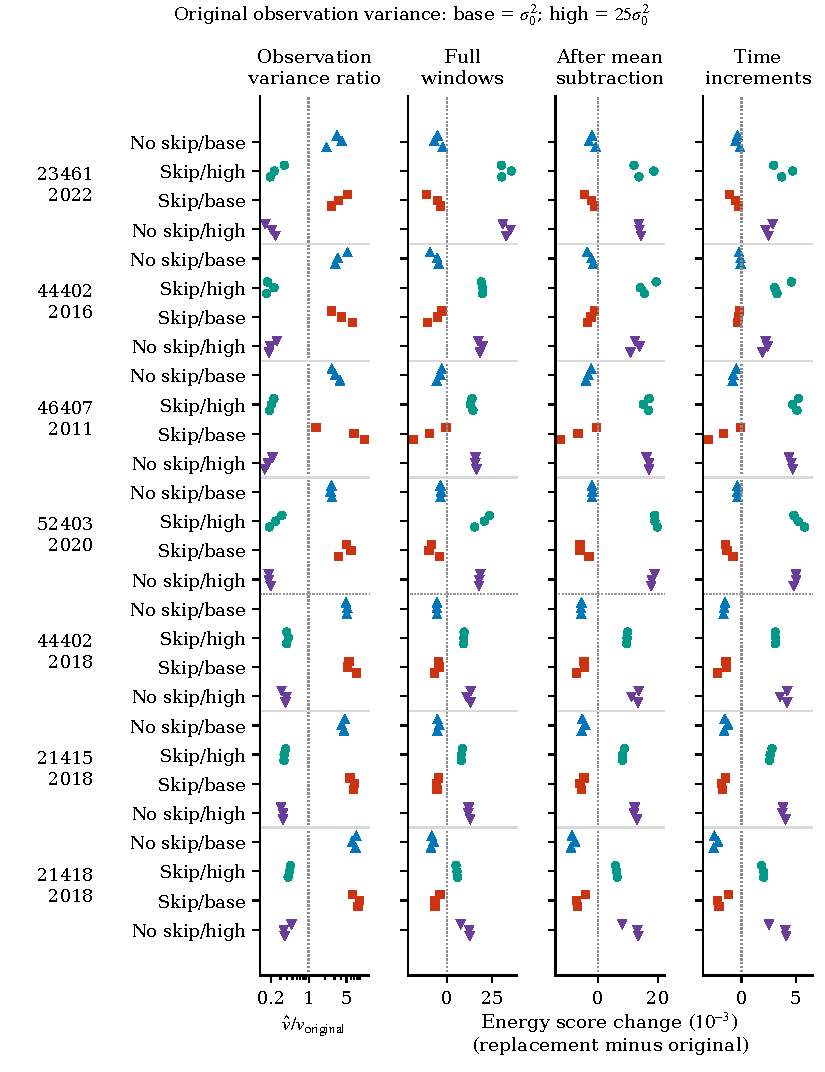
\includegraphics[width=\linewidth,height=0.81\textheight,keepaspectratio]{figures/presentation/dart_variance_refit.pdf}
\caption{Observation variance replacement for all 84 DART fits. Each record and condition has three points, ordered from top to bottom by training seeds 42, 1729, and 31415. The variance ratio is $\hat v/v_{\mathrm{original}}$, with $\hat v$ combining three posterior streams; a ratio of one means equal variances. Energy score columns give $10^3$ times the difference between scores after and before variance replacement in standardized coordinates, averaged over three common prior streams. Negative values indicate lower energy scores after replacement. For each fit, the thin bar spans the smallest to largest score change across the three common sampling streams. Original cases use network weights chosen by validation and equal window weights; 2018 cases use final network weights and UTC start hour weights.}
\label{fig:dart_variance_refit}
\end{figure}

\begingroup
\setlength{\tabcolsep}{3pt}
\begin{longtable}{llrrrr}
\caption{Observation variance estimation on training windows, keeping encoder and decoder weights the same. The variance column gives $10^4\hat v$, where $\hat v$ uses squared standardized units. Energy score columns give $10^3$ times the difference between scores after and before variance replacement in standardized coordinates; negative values indicate lower scores after replacement. Entries give the median across three training seeds after averaging sampling streams, with the full range underneath. Original variance is $10^{-4}$ in A/C and $0.0025$ in B/D. Variance is estimated separately for each model, so the resulting values can differ between conditions.}\label{tab:dart_variance}\\
\toprule
Record & Condition & $10^4\hat v$ & $10^3\Delta$ \shortstack{Full\\windows} & $10^3\Delta$ \shortstack{After mean\\subtraction} & $10^3\Delta$ \shortstack{Time\\increments}\\
\midrule
\endfirsthead
\toprule
Record & Condition & $10^4\hat v$ & $10^3\Delta$ \shortstack{Full\\windows} & $10^3\Delta$ \shortstack{After mean\\subtraction} & $10^3\Delta$ \shortstack{Time\\increments}\\
\midrule
\endhead
23461/2022 & A & \shortstack{3.32\\{[2.14, 4.09]}} & \shortstack{-5.13\\{[-6.91, -2.27]}} & \shortstack{-2.11\\{[-3.1, -0.803]}} & \shortstack{-0.395\\{[-0.559, -0.141]}} \\
23461/2022 & B & \shortstack{5.74\\{[4.84, 8.83]}} & \shortstack{30.4\\{[30.2, 35.7]}} & \shortstack{13.7\\{[12.1, 18.8]}} & \shortstack{3.7\\{[2.97, 4.72]}} \\
23461/2022 & C & \shortstack{3.53\\{[2.63, 5.27]}} & \shortstack{-5.15\\{[-11, -3.29]}} & \shortstack{-2.25\\{[-4.58, -1.3]}} & \shortstack{-0.566\\{[-1.11, -0.32]}} \\
23461/2022 & D & \shortstack{5.18\\{[3.94, 6.08]}} & \shortstack{32.9\\{[31, 35.2]}} & \shortstack{13.9\\{[13.7, 14.4]}} & \shortstack{2.48\\{[2.22, 2.88]}} \\
44402/2016 & A & \shortstack{3.45\\{[3.1, 5.24]}} & \shortstack{-5.3\\{[-9.19, -4.46]}} & \shortstack{-2.22\\{[-3.63, -1.67]}} & \shortstack{-0.105\\{[-0.246, -0.0806]}} \\
44402/2016 & B & \shortstack{4.27\\{[4.14, 5.68]}} & \shortstack{19.7\\{[19.1, 19.8]}} & \shortstack{15.6\\{[14.1, 19.5]}} & \shortstack{3.28\\{[3.04, 4.6]}} \\
44402/2016 & C & \shortstack{4.1\\{[2.66, 6.45]}} & \shortstack{-5.23\\{[-10.7, -2.68]}} & \shortstack{-2.39\\{[-3.57, -1.3]}} & \shortstack{-0.281\\{[-0.395, -0.172]}} \\
44402/2016 & D & \shortstack{4.93\\{[4.55, 6.41]}} & \shortstack{18.4\\{[17.5, 19.9]}} & \shortstack{12.4\\{[10.9, 13.9]}} & \shortstack{2.23\\{[1.94, 2.4]}} \\
46407/2011 & A & \shortstack{3.12\\{[2.7, 3.83]}} & \shortstack{-3.54\\{[-5.57, -2.85]}} & \shortstack{-3.3\\{[-4.05, -2.28]}} & \shortstack{-0.76\\{[-0.828, -0.486]}} \\
46407/2011 & B & \shortstack{5.07\\{[4.72, 5.65]}} & \shortstack{14\\{[12.9, 14.5]}} & \shortstack{16.9\\{[15.2, 17.1]}} & \shortstack{5.13\\{[4.72, 5.24]}} \\
46407/2011 & C & \shortstack{6.91\\{[1.36, 10.8]}} & \shortstack{-9.52\\{[-18.3, -0.433]}} & \shortstack{-6.68\\{[-12.6, -0.418]}} & \shortstack{-1.68\\{[-3.08, -0.119]}} \\
46407/2011 & D & \shortstack{4.39\\{[3.84, 5.29]}} & \shortstack{15.9\\{[15.8, 16.5]}} & \shortstack{17.1\\{[16.3, 17.1]}} & \shortstack{4.59\\{[4.39, 4.73]}} \\
52403/2020 & A & \shortstack{2.65\\{[2.56, 2.7]}} & \shortstack{-3.36\\{[-3.43, -3.07]}} & \shortstack{-2.01\\{[-2.08, -1.94]}} & \shortstack{-0.388\\{[-0.408, -0.386]}} \\
52403/2020 & B & \shortstack{6.09\\{[4.62, 7.94]}} & \shortstack{20.8\\{[15.4, 23.6]}} & \shortstack{19.1\\{[19, 19.9]}} & \shortstack{5.23\\{[4.84, 5.83]}} \\
52403/2020 & C & \shortstack{4.99\\{[3.54, 6.07]}} & \shortstack{-8.48\\{[-9.78, -4.19]}} & \shortstack{-6.09\\{[-6.1, -3.05]}} & \shortstack{-1.37\\{[-1.49, -0.785]}} \\
52403/2020 & D & \shortstack{4.55\\{[4.52, 4.92]}} & \shortstack{18\\{[17.9, 18.5]}} & \shortstack{18.1\\{[17.8, 19]}} & \shortstack{5.03\\{[4.81, 5.05]}} \\
44402/2018 & A & \shortstack{5.09\\{[4.89, 5.18]}} & \shortstack{-5.38\\{[-5.48, -5.3]}} & \shortstack{-5.64\\{[-5.72, -5.57]}} & \shortstack{-1.62\\{[-1.67, -1.55]}} \\
44402/2018 & B & \shortstack{9.8\\{[9.71, 10.5]}} & \shortstack{9.4\\{[9.27, 9.62]}} & \shortstack{9.75\\{[9.6, 9.91]}} & \shortstack{3.12\\{[3.11, 3.15]}} \\
44402/2018 & C & \shortstack{5.55\\{[5.25, 7.79]}} & \shortstack{-4.42\\{[-6.96, -4.36]}} & \shortstack{-4.74\\{[-7.25, -4.57]}} & \shortstack{-1.44\\{[-2.25, -1.38]}} \\
44402/2018 & D & \shortstack{9.21\\{[7.83, 9.58]}} & \shortstack{13.1\\{[10.9, 13.2]}} & \shortstack{13.5\\{[11.2, 13.7]}} & \shortstack{4.22\\{[3.54, 4.22]}} \\
21415/2018 & A & \shortstack{4.52\\{[4.1, 4.66]}} & \shortstack{-5.15\\{[-5.22, -4.06]}} & \shortstack{-5.34\\{[-5.47, -4.26]}} & \shortstack{-1.57\\{[-1.61, -1.25]}} \\
21415/2018 & B & \shortstack{8.76\\{[8.73, 9.4]}} & \shortstack{8.17\\{[8, 8.65]}} & \shortstack{8.29\\{[8.15, 8.84]}} & \shortstack{2.64\\{[2.6, 2.82]}} \\
21415/2018 & C & \shortstack{6.81\\{[5.84, 7.06]}} & \shortstack{-5.39\\{[-5.67, -4.62]}} & \shortstack{-5.62\\{[-6.02, -4.77]}} & \shortstack{-1.76\\{[-1.87, -1.51]}} \\
21415/2018 & D & \shortstack{8.3\\{[7.68, 8.36]}} & \shortstack{12.2\\{[11.9, 12.9]}} & \shortstack{12.3\\{[12, 13]}} & \shortstack{3.85\\{[3.76, 4.05]}} \\
21418/2018 & A & \shortstack{7.39\\{[6.39, 7.64]}} & \shortstack{-8.32\\{[-8.61, -7.26]}} & \shortstack{-8.75\\{[-9.1, -7.73]}} & \shortstack{-2.54\\{[-2.58, -2.17]}} \\
21418/2018 & B & \shortstack{11.1\\{[10.4, 11.4]}} & \shortstack{5.64\\{[5.16, 5.96]}} & \shortstack{6.23\\{[5.8, 6.43]}} & \shortstack{2.02\\{[1.84, 2.03]}} \\
21418/2018 & C & \shortstack{8.19\\{[6.52, 8.87]}} & \shortstack{-6.44\\{[-6.53, -3.73]}} & \shortstack{-6.82\\{[-7.33, -4.11]}} & \shortstack{-2.08\\{[-2.23, -1.21]}} \\
21418/2018 & D & \shortstack{8.93\\{[8.68, 12]}} & \shortstack{12.3\\{[7.71, 12.7]}} & \shortstack{13.2\\{[8.09, 13.6]}} & \shortstack{4.04\\{[2.54, 4.11]}}
\\
\bottomrule
\end{longtable}
\endgroup

\clearpage
\subsection{Network weights, window weights, and variation through time}
An additional evaluation of the 2018 models uses network weights chosen by validation energy score and separate prior and IW streams. These samples differ from those used for final weights even when validation chooses step 10,000. The comparison with equal window weights reuses the primary scores at final weights. Both comparisons were specified before inspection of the new test results.

\begingroup
\setlength{\tabcolsep}{1.3pt}
\begin{longtable}{lllrrrr}
\caption{Alternative network and window weights for the three 2018 records. Entries give the median energy score difference across three training seeds and the full range, comparing conditions with the same seed. Negative values favor the skip. Selected/UTC uses network weights chosen by validation and equal total window weight in each UTC start hour. Final/uniform uses final network weights and equal window weights. Steps gives the minimum and maximum Adam step counts across both conditions and all seeds, or their common final count. Streams are averaged within fits. Evaluations at weights chosen by validation and at final weights use different samples. C-A and B-D use the same original observation variance within each comparison.}\label{tab:dart_selected}\\
\toprule
Record & $\Delta$ & Evaluation & Steps & \shortstack{Full\\windows} & \shortstack{After mean\\subtraction} & \shortstack{Time\\increments}\\
\midrule
\endfirsthead
\toprule
Record & $\Delta$ & Evaluation & Steps & \shortstack{Full\\windows} & \shortstack{After mean\\subtraction} & \shortstack{Time\\increments}\\
\midrule
\endhead
44402/2018 & C-A & Selected/UTC & 6000--10000 & \shortstack{-0.359\\{[-0.748, -0.128]}} & \shortstack{-0.385\\{[-0.519, -0.298]}} & \shortstack{-0.0368\\{[-0.055, -0.0353]}} \\
44402/2018 & C-A & Final/uniform & 10000 & \shortstack{-0.337\\{[-0.768, -0.119]}} & \shortstack{-0.346\\{[-0.479, -0.296]}} & \shortstack{-0.035\\{[-0.0522, -0.0334]}} \\
44402/2018 & B-D & Selected/UTC & 10000--10000 & \shortstack{-0.262\\{[-0.33, -0.241]}} & \shortstack{-0.239\\{[-0.37, -0.201]}} & \shortstack{-0.0288\\{[-0.0431, -0.0213]}} \\
44402/2018 & B-D & Final/uniform & 10000 & \shortstack{-0.222\\{[-0.322, -0.219]}} & \shortstack{-0.227\\{[-0.363, -0.151]}} & \shortstack{-0.0267\\{[-0.0419, -0.0157]}} \\
21415/2018 & C-A & Selected/UTC & 8000--10000 & \shortstack{-0.328\\{[-0.334, -0.255]}} & \shortstack{-0.406\\{[-0.409, -0.317]}} & \shortstack{-0.06\\{[-0.0612, -0.0448]}} \\
21415/2018 & C-A & Final/uniform & 10000 & \shortstack{-0.299\\{[-0.35, -0.211]}} & \shortstack{-0.371\\{[-0.377, -0.331]}} & \shortstack{-0.0555\\{[-0.0562, -0.0473]}} \\
21415/2018 & B-D & Selected/UTC & 10000--10000 & \shortstack{-0.267\\{[-0.335, -0.228]}} & \shortstack{-0.266\\{[-0.329, -0.204]}} & \shortstack{-0.0397\\{[-0.0526, -0.0314]}} \\
21415/2018 & B-D & Final/uniform & 10000 & \shortstack{-0.248\\{[-0.345, -0.225]}} & \shortstack{-0.247\\{[-0.324, -0.212]}} & \shortstack{-0.0364\\{[-0.0519, -0.0328]}} \\
21418/2018 & C-A & Selected/UTC & 9000--10000 & \shortstack{-0.638\\{[-0.82, -0.282]}} & \shortstack{-0.463\\{[-0.633, -0.409]}} & \shortstack{-0.0587\\{[-0.0918, -0.0535]}} \\
21418/2018 & C-A & Final/uniform & 10000 & \shortstack{-0.61\\{[-0.856, -0.262]}} & \shortstack{-0.45\\{[-0.631, -0.407]}} & \shortstack{-0.0573\\{[-0.091, -0.0541]}} \\
21418/2018 & B-D & Selected/UTC & 10000--10000 & \shortstack{-0.462\\{[-0.577, -0.453]}} & \shortstack{-0.508\\{[-0.553, -0.366]}} & \shortstack{-0.0689\\{[-0.0755, -0.0533]}} \\
21418/2018 & B-D & Final/uniform & 10000 & \shortstack{-0.473\\{[-0.557, -0.424]}} & \shortstack{-0.499\\{[-0.535, -0.355]}} & \shortstack{-0.0683\\{[-0.0724, -0.0521]}}
\\
\bottomrule
\end{longtable}
\endgroup

Variation through time is summarized in intervals of 14 days and 28 days, measured from the start of the first retained training window. Each test window belongs to the interval containing its start time. An interval's total weight is the sum of its window weights. Multiplying its weighted mean score by that total gives its contribution to the overall mean; all contributions sum to that mean. The calculation includes intervals with few windows and windows that extend beyond an interval's end. Table~\ref{tab:dart_blocks} gives ranges of differences between conditions on the same intervals across three training seeds. Population confidence intervals would require an inference method that accounts for serial dependence and sparse coverage.

Adjacent 2018 windows starting four hours apart share 176 of 192 observations. The split exclusions prevent observations from appearing in more than one partition. Within partitions, overlap and recurring oscillations preserve dependence. All three scores use the same windows. For 21415 and 21418, some intervals of 14 days favor the model without a skip, whereas the full test partitions and all intervals of 28 days that contain data favor the skip.

\begin{table}[H]
\centering
\setlength{\tabcolsep}{3pt}
\caption{Ranges of energy score differences on full windows, in standardized coordinates, across training seeds and across intervals of 14 days and 28 days that contain test windows. Negative differences favor the skip. Intervals gives the number of intervals of each length that contain test windows. Serial dependence remains. C-A compares skip with no skip at base variance; B-D makes the same comparison at high variance. Each interval score averages three sampling streams using the record's window weights.}\label{tab:dart_blocks}
\begin{tabular}{llrrrr}
\toprule
Record & Intervals & \shortstack{C-A\\14 days} & \shortstack{C-A\\28 days} & \shortstack{B-D\\14 days} & \shortstack{B-D\\28 days}\\
\midrule
23461/2022 & 3/2 & [-1.21, 1.53] & [-1.21, 1.51] & [0.77, 3.41] & [0.77, 3.4] \\
44402/2016 & 6/4 & [-1.41, 0.87] & [-1.41, 0.861] & [0.096, 0.221] & [0.096, 0.221] \\
46407/2011 & 5/3 & [-1.19, 0.991] & [-1.19, 0.962] & [-0.497, 0.204] & [-0.497, 0.195] \\
52403/2020 & 4/3 & [-0.917, 0.805] & [-0.917, 0.805] & [-0.634, 3.25] & [-0.634, 3.25] \\
44402/2018 & 5/3 & [-0.799, -0.0818] & [-0.795, -0.103] & [-0.34, -0.175] & [-0.34, -0.206] \\
21415/2018 & 5/3 & [-0.914, 0.465] & [-0.393, -0.141] & [-0.709, 0.0503] & [-0.403, -0.217] \\
21418/2018 & 5/3 & [-0.903, 0.0589] & [-0.872, -0.25] & [-0.67, 0.0133] & [-0.575, -0.408]
\\
\bottomrule
\end{tabular}
\end{table}

\clearpage
\section{Feature ECDFs and spectra}
Figures~\ref{fig:dart_ecdf_historical} to~\ref{fig:dart_spectra_fresh} use the same fitted models and prior samples at the original observation variance as the DART energy score evaluation. Training and test windows use their own partition weights: uniform for the original records and equal mass in each UTC start hour for 2018. Generated samples have equal weight. For each neural fit, feature or power calculations use three streams of 1,024 samples. Their empirical cumulative distribution functions (ECDFs) or bin powers are then averaged. At each feature value or frequency, curves give the median across three training seeds and shading spans their full range. A curve constructed this way can combine values from different fits. PPCA is one baseline fit, with its curve averaging three sampling streams.

The ECDFs use three features: the difference between window mean and training mean, standard deviation (SD) within a window, and the Euclidean norm of the vector of time increments in Eq.~\ref{eq:increments}. Multiplication by the training scale expresses feature values in meters. For values $a_i$, the ECDF is $\widehat F(t)=\sum_i\tilde w_i\mathbf{1}\{a_i\le t\}$, with weights summing to one within each observation partition or generated sample set. All ties at exact feature values remain. Each ECDF describes one feature. Agreement of these feature distributions still allows different joint distributions of the window coordinates and different relations between mean and shape.

Each spectrum uses 192 observations after subtraction of their window mean, with equal weight at every position. The one-sided power spectrum calculated from the discrete Fourier transform (DFT) combines power at positive and negative frequencies: interior positive bins contribute twice, while the Nyquist bin contributes once. The 96 positive bins run from 0.5 to 48 cycles/day. Their powers, in square meters per bin, sum to the window's variance; division by the bin width would give power spectral density. Powers are averaged in linear units and displayed on logarithmic axes. The median is then taken separately at each frequency across training seeds, so its sum can differ from the median variance of the fits. Dashed neural curves use decoder means from prior latent samples. These spectra describe variation within windows and omit differences in window means. Subtracting each window's mean preserves tidal oscillations; nearby constituents remain unresolved at the 0.5 cycle per day bin spacing.

On the 2018 records, neural prior samples vary less within windows than the observations: both their standard deviations and norms of time increments are smaller. Their spectra contain less power in the prominent low-frequency peaks and, in several conditions, more power at high frequencies. PPCA reproduces more of the variation, although its feature distributions also differ from the data; at 44402/2018, it gives a broader distribution of window standard deviations. Architecture, the variational family, and training all differ between PPCA and the neural fits, so their separate contributions remain unresolved.

\begin{figure}[p]
\centering
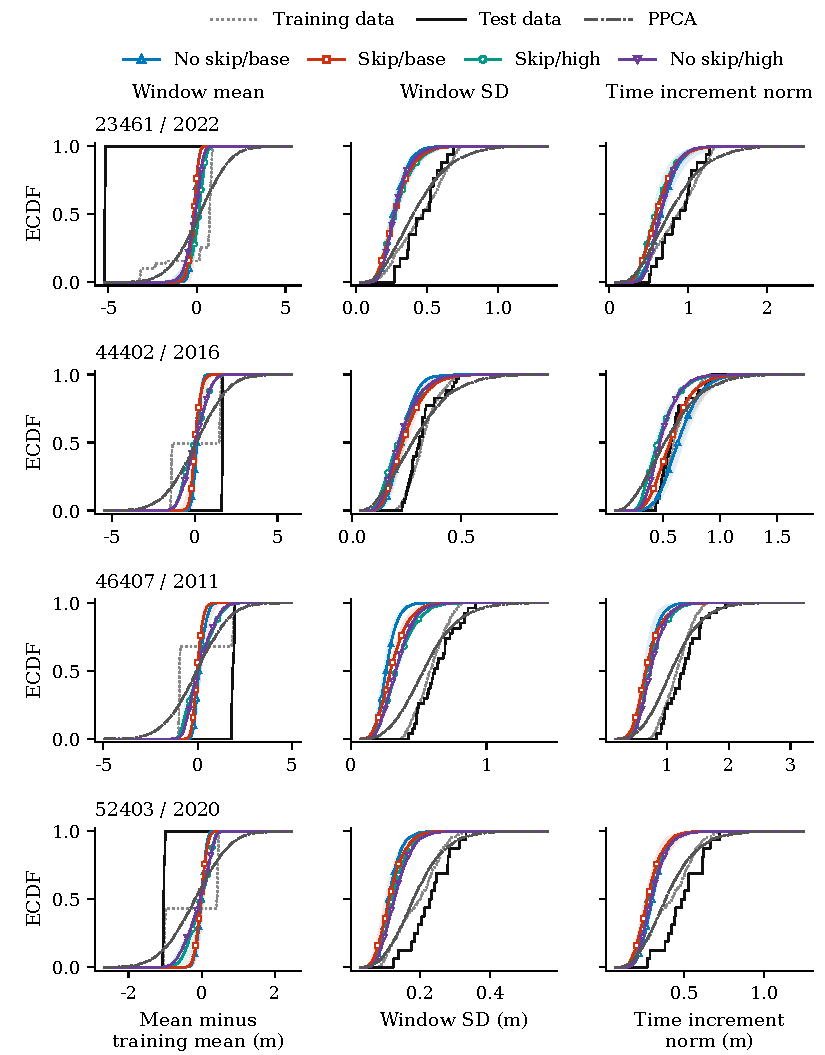
\includegraphics[width=\linewidth,height=0.81\textheight,keepaspectratio]{figures/presentation/dart_ecdf_historical.pdf}
\caption{Feature ECDFs for the four original DART records: observed training and test windows, noisy prior samples from conditions A--D, and PPCA. At each feature value, neural curves give the median across three fits per condition at the weights chosen by validation, after averaging three sampling streams within each fit. Shading spans the full range across training seeds. Observed windows have equal weights. Each stream contains 1,024 prior samples.}
\label{fig:dart_ecdf_historical}
\end{figure}

\begin{figure}[p]
\centering
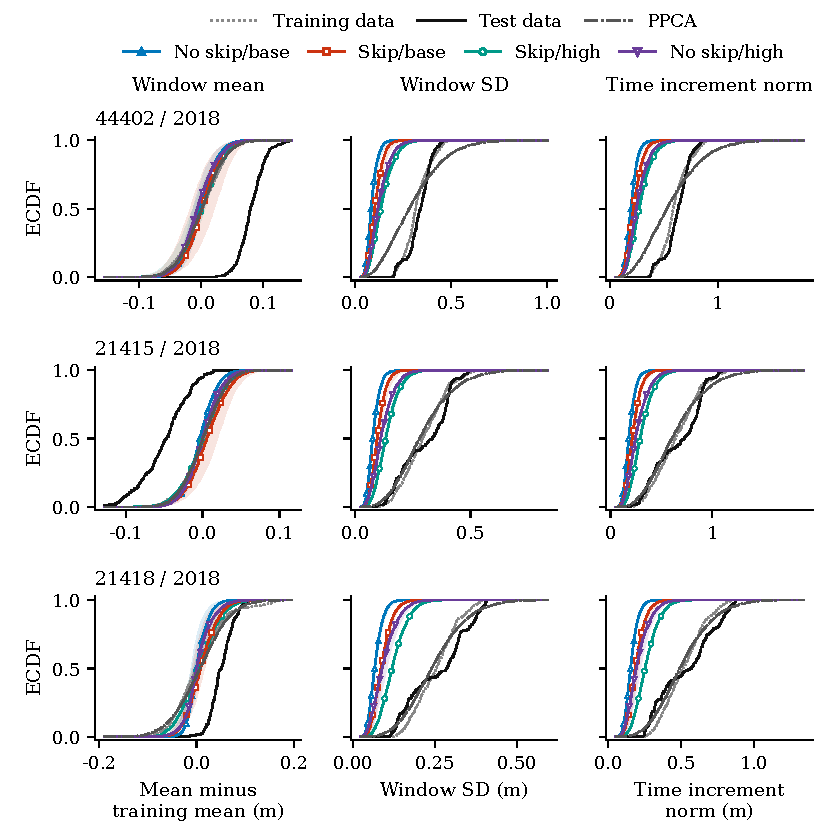
\includegraphics[width=\linewidth,height=0.81\textheight,keepaspectratio]{figures/presentation/dart_ecdf_fresh.pdf}
\caption{Feature ECDFs for the three additional DART records. Observed training and test windows use their respective UTC start hour weights. Generated samples have equal weight. At each feature value, neural curves give the median across three final fits per condition, after averaging three streams within each fit. Shading spans the full range across training seeds. The PPCA curve averages three sampling streams from one baseline fit.}
\label{fig:dart_ecdf_fresh}
\end{figure}

\begin{figure}[p]
\centering
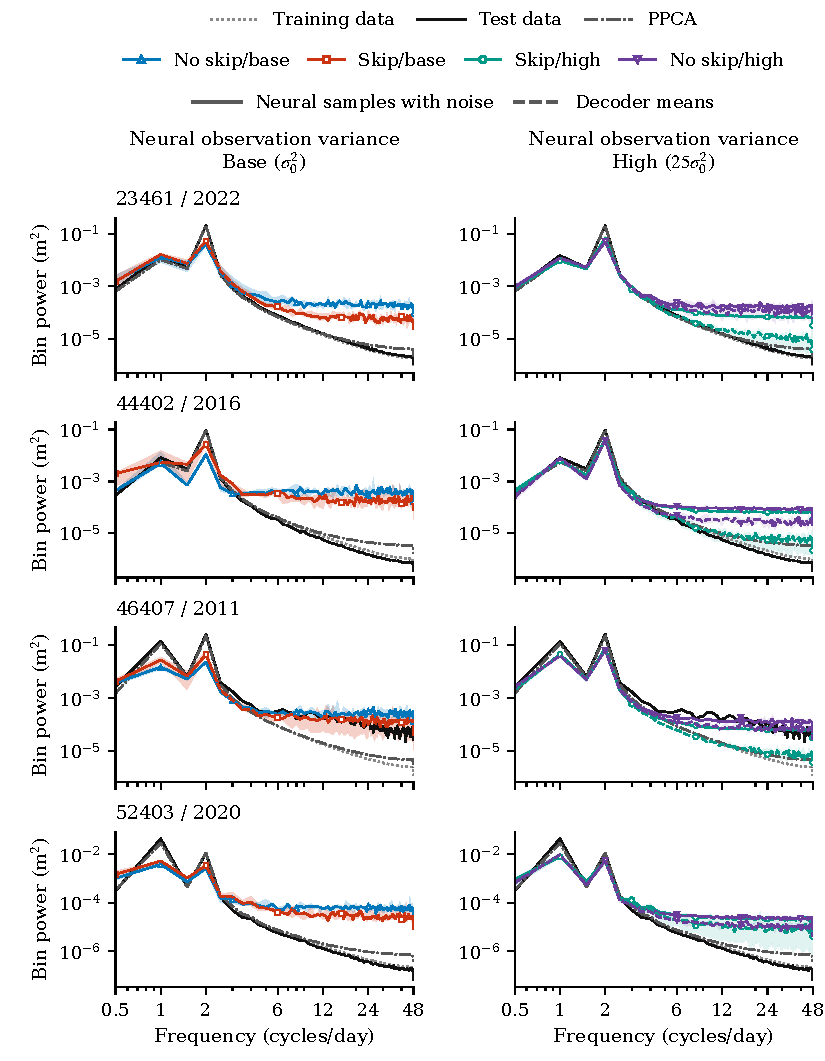
\includegraphics[width=\linewidth,height=0.81\textheight,keepaspectratio]{figures/presentation/dart_spectra_historical.pdf}
\caption{DFT bin powers within windows for the four original records. The base variance columns use $\sigma_0^2$ and high variance columns use $25\sigma_0^2$, with observed training and test windows and PPCA in each column. Solid neural curves include observation noise; dashed curves use decoder means from prior latent samples. Neural fits use weights chosen by validation. Each fit's bin powers are averaged over three streams in linear units, followed by the median and full range across training seeds at each frequency. Both columns use the same PPCA fit. Each window's mean is subtracted before the DFT, excluding variation of means. Both axes are logarithmic. The 0.5 cycle per day bin spacing leaves nearby tidal constituents unresolved.}
\label{fig:dart_spectra_historical}
\end{figure}

\begin{figure}[p]
\centering
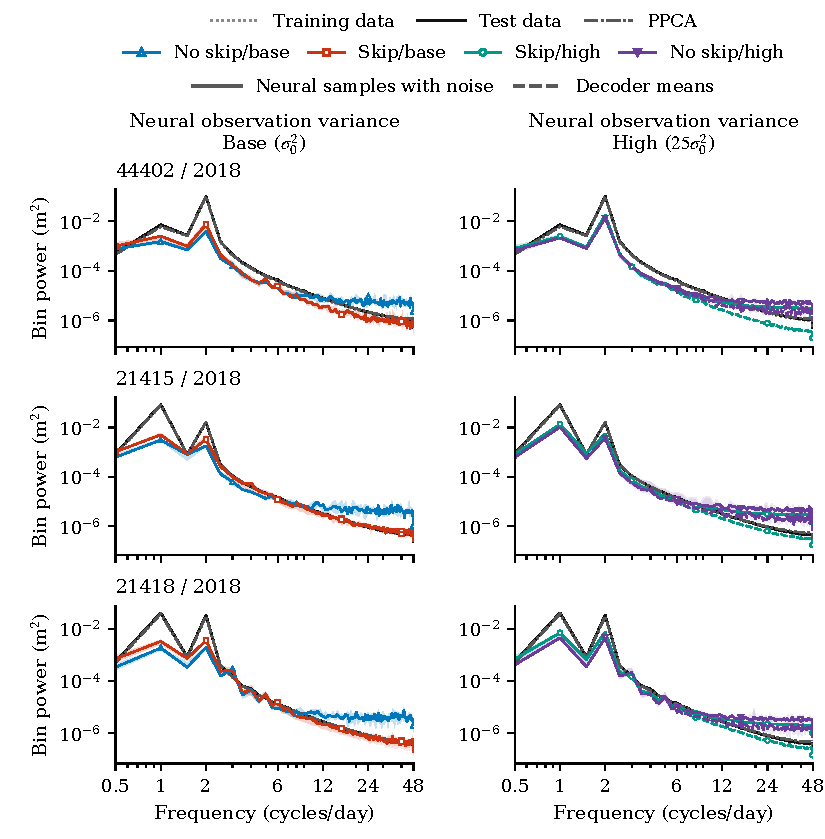
\includegraphics[width=\linewidth,height=0.81\textheight,keepaspectratio]{figures/presentation/dart_spectra_fresh.pdf}
\caption{DFT bin powers within windows for the three additional records. Training and test spectra use the UTC start hour weights for their respective partitions. Neural curves use final fits at original variance: solid curves include observation noise and dashed curves use decoder means from prior latent samples. Each fit's bin powers are averaged over three streams in linear units, followed by the median and full range across training seeds at each frequency. Both columns use the same PPCA fit. Each window's mean is subtracted before the DFT. Both axes are logarithmic. The 0.5 cycle per day bin spacing leaves nearby tidal constituents unresolved.}
\label{fig:dart_spectra_fresh}
\end{figure}
\clearpage

\section{Records, tides, and HEIGHT}
\label{sec:scope}
The seven DART records cover six sites, including two years from 44402. The original records contribute 95 test windows and the additional records contribute 773 overlapping test windows. Serial dependence persists within these observations. The comparisons describe the available station records under the data selection and fitting procedures above.

The four original DART records were chosen and inspected before this evaluation. NCEI lists deployment dates of April 23, 2016 for 44402 \citep{NCEIDART44402}, May 29, 2011 for 46407 \citep{NCEIDART46407}, and August 13, 2020 for 52403 \citep{NCEIDART52403}. Deployments can involve sensor replacement and recalibration. Each date precedes the corresponding training cutoff, so three training partitions span deployments while validation and test use subsequent observations. Establishing the causes of height changes requires evidence beyond deployment dates. Drift, environmental variability, data availability, and the reporting types included can also alter the distribution within a deployment.

Within each uninterrupted segment of an original record, training windows start four hours apart and evaluation windows 48 hours apart. Over 48 hours the solar semidiurnal S2 phase repeats, the lunisolar diurnal K1 phase nearly repeats, and the lunar semidiurnal M2 phase advances appreciably. Segment breaks can change the starting phase. Normalization uses every retained training row once, including fragments too short to form windows, whereas overlapping training windows reuse observations and test windows receive equal weights. The split exclusions keep source observations in separate partitions. Tidal and longer temporal dependence can still extend across them.

HEIGHT expresses bottom pressure as equivalent water column height after compensation for sensor temperature effects, using 670 mm per pound per square inch absolute (PSIA) \citep{NDBCDARTDescription,Meinig2005DARTII}. The conversion is nominal: surveyed instrument depth and surface elevation are different physical quantities. NOAA describes measurements every 15 seconds and routine spot values from those data at intervals of 15 minutes. Meinig et al.\ describe nominal integration over 15 seconds and separately call the transmitted height an ``average'' \citep[Sections 3.3.1, 3.3.2, and 3.3.8]{Meinig2005DARTII}. Applying these system descriptions to a particular annual record also requires its firmware and timestamp conventions. Within each retained routine window, observations are 900 s apart. Excluding event reporting types can also affect which physical conditions enter the analysis.

The 900 s spacing gives a Nyquist frequency of 48 cycles/day, corresponding to a period of 30 minutes. A DFT of 192 observations has bins 0.5 cycles/day apart. Peaks near diurnal and semidiurnal frequencies can be compared, but nearby constituents remain unresolved: the M2/S2 and K1/O1 beat periods are about 14.8 and 13.7 days \citep{NOAA2000TideGlossary}. O1 is the lunar diurnal constituent. Harmonic fitting estimates amplitudes and phases at known constituent frequencies; the DFT plots report power in frequency bins. The reliability of harmonic fitting depends on record length, constituent separation, and noise \citep{Parker2007TidalAnalysis}. Coefficients from a longer calibration record can be applied to shorter windows.

Instrument sensitivity and the sampling interval impose separate limits. \citet{EbleGonzalez1991BottomPressure} measured deep-ocean bottom pressure at 64 samples per hour and described millimeter scale sensitivity in principle for oscillations longer than a few minutes, with practical resolution limited by drift and background noise. Deep water attenuates the bottom pressure response to ordinary wind waves and swell \citep[Section 2.2.1]{Meinig2005DARTII}. Interpreting power at high frequencies requires accounting for both the pressure response at the instrument's depth and the effects of finite sampling. These experiments assess distributions of routine windows. Noise removal, anomaly classification, and operational warning are separate tasks whose evaluation needs independent evidence about the events or measurement errors of interest.

\end{document}
